\documentclass[article,11pt]{revtex4}
%\documentclass[twocolumn,prb]{revtex4}
\usepackage{epsfig,amsmath,amssymb,color}
\bibliographystyle{apsrev}
\newcommand{\mohammad}[1]{\textcolor{red}{#1}}
\newcommand{\adrian}[1]{\textcolor{blue}{#1}}
\newcommand{\remove}[1]{\textcolor{black}{#1}}

\usepackage{wrapfig}
%\bibliography{si-gs,dmrg}

%\voffset1.2cm
\begin{document}


\title{Interplay between charge, spin, and phonons in low dimensional strongly interacting systems}
\author{Mohammad Soltanieh-ha}
\affiliation{Department of Physics, Northeastern University, Boston, Massachusetts 02115, USA}
%\author{PI:  Prof. \hspace*{-.15in} Adrian E. Feiguin}
%\date{\today}
\vspace*{-.75in}
\maketitle
\vspace*{-.3in}
\hspace*{.in}
\textbf{Committee Members} \\
\hspace*{0.5in}Prof. Adrian E. Feiguin (Advisor)\\% \hfill 
\hspace*{0.5in}Prof. Arun Bansil  \hspace*{.24in}    \\
\hspace*{0.5in}Prof. Robert Markiewicz\\%  \hfill 
\hspace*{0.5in}Prof. Donald Heiman
\vspace*{-.5in}
\tableofcontents

\section{Introduction}

\subsection {Interacting systems in low dimensions}

%One-dimensional systems of interacting particles are particularly interesting since interactions behave non-perturbatively due to the pervasive nesting existing at all densities. This means that interactions cannot be treated withing Fermi liquid theory, as we usually do in higher dimensions, not even for small interactions. Furthermore, the natural excitations in one dimensional systems are collective modes, and bosonic in nature, meaning that the quasi-particle paradigm breaks down. Such systems of correlated particles have been studied theoretically for over 50 years, and have been the driving force behind Luttinger Liquid theory and conformal field theory. In some cases one might be able to obtain a complete and exact solution of a problem using Bethe ansatz \cite{TakahashiBook}. 

The physics of correlated low dimensional systems is quite different than their higher dimensional counterparts. In three-dimensions, the physics can be described within Fermi liquid theory, where there is a one-to-one correspondence
between the excitations of a weakly interacting Fermi system, so-called
quasi-particles, and the excitations of a non-interacting one. Quasi-particles preserve the same quantum numbers as the original excitations in the original system. This scenario breaks down in one dimension (1D): in
this case, the Fermi surface reduces to two points in momentum space, at
$k=\pm k_F$, and the resulting nesting, pervasive at all densities,
prevents the application of perturbation theory. This leads to a
new paradigm: the Luttinger liquid \cite{Haldane1981,Gogolin,GiamarchiBook}. In a Luttinger liquid (LL), the natural
excitations are collective density fluctuations, that carry either spin
(``spinons''), or charge (``holons''). These excitations have different
dispersions, and obviously, do not carry the same quantum numbers as the
original fermions. This leads to the spin-charge separation (SCS) picture, in
which a fermion injected into the system breaks down into excitations carrying different quantum numbers, each with a characteristic energy scale and velocity (one for the charge, one for the spin).

 Such systems of correlated particles have been studied theoretically for over 50 years, and have been the driving force behind Luttinger Liquid theory, bosonization, and conformal field theory. In some cases one might be able to obtain a complete and exact solution of a problem using Bethe ansatz \cite{TakahashiBook}. 

We began to see experimental realizations of the one-dimesional behavior in isolated 1D and also bulk materials in the 1970's with polymers and organic compounds. Some of them are organic superconductors \cite{ChemRev}, ladder compounds \cite{Dagotto1996}, quantum wires \cite{Fisher1997}, carbon nanotubes \cite{Dress1995}, edge states in quantum hall systems \cite{Pitaevskii,Greiner} to mention a few \cite{GiamarchiBook}.

Recently, a previously overlooked regime at finite temperature has come to
light: the ``spin-incoherent Luttinger liquid'' (SILL) \cite{Matveev2004,Fiete2004,Cheianov2004,Cheianov2005,Fiete2007b,Halperin2007}.
Due to the fact that the holons and spinons have independent energy scales, their behavior at finite temperature will be quite different. 
If the spinon bandwidth is much smaller than the holon bandwidth, a small temperature relative to the Fermi energy may actually be felt as a very large temperature by the spins. In fact, the charge will remain very close to the {\it charge} ground-state, but the spins will become totally incoherent, effectively at infinite temperature.
 This regime is characterized by universal properties in the transport, tunneling density of states, and the spectral functions \cite{Fiete2007b}, and will occupy a great deal of our attention in the rest of our discussion.

In Ref.\onlinecite{Feiguin2009d}, it was shown how this crossover from spin-coherent to spin-incoherent is characterized by a transfer of spectral weight. Remarkably, the photoemission spectrum of the SILL can be understood by assuming that after the spin is thermalized, the charge becomes spinless, with a shift of the Fermi momentum from $k_F$ to $2k_F$. In a follow-up paper \cite{Feiguin2011}, it was shown that a coupling to a spin bath can have a similar effect as temperature, but in the ground-state. The ``spin-incoherent'' ground-state will have the same qualitative features as the SILL at finite temperature. In the next few chapters we formalize this conjecture into a unified theory that describes the spin-incoherent ground-state for a variety of model Hamiltonians, such as the $t-J$-Kondo chain and $t-J$ ladders \cite{Soltanieh-ha2012}. The main ingredient for the validity of this theory is to have a very flat spinon dispersion, which corresponds to the limit in which spin and charge completely decouple from each other. This formalism is exact in this limit, and provides a new theoretical framework to understand spin-incoherent physics, including the structure of the Kondo lattice ground-state and entanglement.

\subsection {The Hubbard and the $t-J$ Hamiltonian models}

The one-dimensional Hubbard Hamiltonian is a paradigmatic model in condensed matter, not only for its relative simplicity, but mainly because it contains the basic ingredients to understand the physics emerging from strong interactions. Moreover, its higher dimensional counterpart has been assummed for decades to be the minimal model that can explain high temperature superconductivity, and has acquired even more relevance recently in view of the current efforts to realize it in cold atomic systems. 

The model can be exactly solved by Bethe Ansatz, and its low energy physics can be understood in terms of Luttinger liquid (LL) theory\cite{Haldane1981,Gogolin,GiamarchiBook}. 
In a Luttinger liquid, the natural
excitations are collective density fluctuations, that carry either spin
(``spinons''), or charge (``holons''). This leads to the spin-charge separation picture, in
which a fermion injected into the system breaks down into excitations carrying different quantum numbers, each with a characteristic energy scale and velocity (one for the charge, one for the spin).

The Hubbard model is the simplest model of interacting particles in a lattice, containing a kinetic term allowing the particles to tunnel through the lattice sites (hopping), and a potential energy term consisting of an on-site interaction \cite{J_Hubbard1963}.  We start by considering an isolated chain of strongly interacting fermions, described by a Hubbard Hamiltonian in one dimension:
\begin{equation}
H=-t \sum_{i=1,\sigma}^L \left(c^\dagger_{i\sigma} c_{i+1\sigma}+\mathrm{h.c.}\right)
+ U \sum_{i=1}^L n_{i,\uparrow} n_{i,\downarrow}.
\label{H_Hub}
\end{equation}
Here, $c^\dagger_{i\sigma}$ $(c_{i\sigma})$ creates (destroys) an electron of spin $\sigma$ on the
$i^{\rm th}$ site along a chain of length $L$, $n_i$ is the particle number operator.

For strong interactions, one can project out double occupancy, and map the problem onto an effective low energy theory described by the so-called $t-J$ model:
\begin{equation}
H=-t \sum_{i=1,\sigma}^L \left(c^\dagger_{i\sigma} c_{i+1\sigma}+\mathrm{h.c.}\right)
+ J \sum_{i=1}^L (\vec{S}_i \cdot \vec{S}_{i+1} -\frac{1}{4} n_i n_{i+1} ),
\label{H_t-J}
\end{equation}
where $\vec{S}_i$ is the spin operator, $J=4t^2/U$, and we consider the implicit constraint forbidding double-occupancy. This means that the hopping term cannot create a particle on an orbital that was previously occupied by a fermion with the opposite spin. 
 The exchange energy between spins is parametrized by $J$. Unless otherwise specified, we express all energies in units of the hopping parameter $t$. Notice that at half-filling, the system becomes a Mott insulator with one particle per site, and the model reduces to the Heisenberg Hamiltonian.

\pagebreak
\section {Spin-charge separation and the Ogata-Shiba Wave-Function}

In the large $U \rightarrow \infty$ limit (or $J \rightarrow 0$ in the $t-J$ model), the ground-state of these Hamiltonians can be described by Ogata and Shiba's factorized wave-function \cite{Ogata1990},
which is the product of a fermionic wave-function $|\phi\rangle$, and a spin wave-function
$|\chi\rangle$
\begin{equation}
|\mathrm{g.s.}\rangle=|\phi\rangle\otimes |\chi\rangle.
\label{gs}
\end{equation}

The first piece, $|\phi\rangle$, describes the charge degrees of freedom, and is
simply the ground-state of a one-dimensional tight-binding chain of $N$ non-interacting spinless fermions. The spin wave-function $|\chi\rangle$ corresponds to a ``squeezed'' chain of $N$ spins, where all the unoccupied sites have been removed.
In this limit, 
the charge and the spin are governed by independent Hamiltonians.
Since the spin energy scale is determined by $J$, for $J=0$ the spin states are degenerate, and the charge dispersion becomes that of a non-interacting band $\epsilon(k)=-2t\cos(k)$. However, any finite value of $J$ will lift this degeneracy and give the spin excitations a finite bandwidth. Notice that in finite systems, the spin degree of freedom affects the charge through an effective magnetic flux, which in the examples shown here is always identically zero \cite{Caspers1989,Penc1997,Rincon2009}.

\subsection {Generalization of the Ogata-Shiba wave-function to infinite spin temperature}

In order to show that the spin incoherent regime at inifinite spin temperature can be described exactly using a pure state we start by establishing an analogy between (i) a thermal mixed state and (ii) a pure state in an enlarged Hilbert space.  This is the key idea behind the so-called thermo field formalism \cite{Takahashi1975}. 
For illustration purposes, let us first assume that we have two spins $S=1/2$, that we put  into
a maximally entangled state
\begin{equation}
|I_0\rangle = \frac{1}{\sqrt{2}}
\left[|\uparrow,\tilde\downarrow\rangle \pm |\downarrow,\tilde\uparrow\rangle\right],
\label{epr}
\end{equation}
where the sign is irrelevant in the following treatment. We shall assume the first spin is our ``physical'' spin, while the one with a tilde is the ``ancilla'', or impurity spin. It is straightforward to see that the reduced density matrix of the physical spin, after tracing over the ancillary degrees of freedom, is the identity matrix.  Thus, if we assume that the ancilla acts as some sort of effective thermal bath, the physical spin is at infinite temperature.

It is easy to see that the maximally mixed state for a number of spins can be rewritten as:
%\begin{equation}
%%%%%|I \rangle = \prod_i \sum_{s_i} |s_i \tilde{s}_i\rangle = \prod_i
$|I \rangle = \prod_i |I_{0i}\rangle,$
%\label{entangled}
%\end{equation}
defining the maximally entangled state $|I_{0i}\rangle$ of spin $i$ with
its ``ancilla'', as in Eq.(\ref{epr}).
This construction allows one to represent a mixed state of a quantum system as a pure state in an enlarged Hilbert space
and lies at the core of the imaginary-time DMRG \cite{Feiguin2005a}.

Now it is easy to construct a generalization of the Ogata-Shiba wave-function to describe the system at {\it infinite spin temperature}. All we have to do is to add spin ancillas, and replace the spin component in Eq.(\ref{gs}), by the corresponding maximally entangled state, $|I \rangle = \prod_i |I_{0i}\rangle$, $|\psi_{SILL}\rangle=|\phi\rangle \otimes |I\rangle$. Thus, the charge will remain at zero temperature, while the spin component will be effectively at infinite temperature! This state is describing the spin-incoherent regime.

\subsection {Applying the Factorized Wave-Function on Different Hamiltonian Models}

Since the SILL regime can be described by a pure state, it is natural to wonder if there is a parent Hamiltonian for this state. Or at least, we would like to find a model whose ground-state can be associated to a thermal state at finite spin temperature.
Let us assume that we antiferromagnetically couple our 1D chain to a bath of spins in the $J=0$ limit. Regardless of the internal structure and dynamics of the bath, it is easy to realize that the charge will be in principle unaffected by it, while the spin degree of freedom will get entangled into a many-body state with the spins from the bath. If we trace over the bath, we expect the spins of the chain to be at an effective finite temperature, parametrized by the magnitude of the system-bath coupling (even though the entire chain plus bath are in a pure state: the ground state of the Hamiltonian). Therefore, the spins of the chain can be driven incoherent by this interaction, while the charge remains in the ground-state. This physics is completely analogous to the SILL physics at finite temperature. 
%We should point out that the coupling with the bath may introduce a gap in the excitation spectrum, but it is to expect that in the regime of interest the gap would remain exponentially small, with the aforementioned picture basically unchanged (whether there is a gap, and/or a critical value of couplings to open a gap is beyond the scope of this work). 
In Ref.\onlinecite{Feiguin2011} it was numerically shown that this physics is indeed realized in the $t-J$-Kondo chain with strongly correlated conduction electrons, where the Kondo impurities act as an effective spin bath. Later in this work we calculate the exact ground-state of this system in this limit, and also coupled $t-J$ chains, and we show that the structure of the ground-state is quite universal, and indicates the path toward a unified formalism to describe spin-incoherent behavior at zero and finite temperatures.

\subsubsection {Two Coupled $t-J$ Chains}

Let us assume two chains governed by the Hamiltonian (\ref{H_t-J}), and we take the $J \rightarrow 0$. In the limit in which the chains are independent, the exact ground-state will be that of two decoupled factorized wave-functions of the form (\ref{gs}):
\begin{equation}
|\mathrm{g.s.}\rangle=|\mathrm{g.s.}\rangle_1 \otimes |\mathrm{g.s.}\rangle_2=|\phi\rangle_1 \otimes |\phi\rangle_2 \otimes |\chi\rangle_1 \otimes |\chi\rangle_2,
\label{gs2}
\end{equation}
where the subindex $\lambda=1,2$ refers to the chain index.
Now we introduce a small but finite antiferromagnetic interaction between the chains of the form
\begin{equation}
H'=J'\sum_{i=1}^L  \vec{s}_{i,1} \cdot \vec{s}_{i,2},
\end{equation}
where $J'$ parametrizes the interaction perpendicular to the direction of the chains, along the rungs of a ladder. This is equivalent to a $t-J$ ladder without inter-chain hopping. We acknowledge that this is a very idealized scenario, since the presence of exchange always implies the existence of a hopping, since $J' \sim t'^2$. Still, this could be considered a model for a two band problem with a Hund coupling, as studied in Ref.\cite{Tsvelik}. It is to expect that this interaction will couple the spin pieces of the wave-function $|\chi\rangle_1$ and $|\chi\rangle_2$, leaving the charge unaltered:
\begin{equation}
|\mathrm{g.s.}\rangle=|\phi\rangle_1 \otimes |\phi\rangle_2 \otimes |S\rangle,
\label{gs3}
\end{equation}
where $|S\rangle$ represents the many body state of the spins for the two coupled chains, once they become entangled by action of the Hamiltonian $H'$.
It is also to expect that this state $|S\rangle$ will be a singlet. However, the exact structure of this singlet is not necessarily trivial. 

Without attempting to deduce the exact effective Hamiltonian for the spin sector, we shall propose a variational ansatz for the wave-function, that we later prove to be exact by numerical means. We argue that every time two spins interact on a rung via $H'$, they will become entangled forming a singlet. Since the interaction along the chain is set to $J=0$, these spins will remain entangled as they move apart from each other by action of the hopping term.

\begin{centering}
\begin{figure}
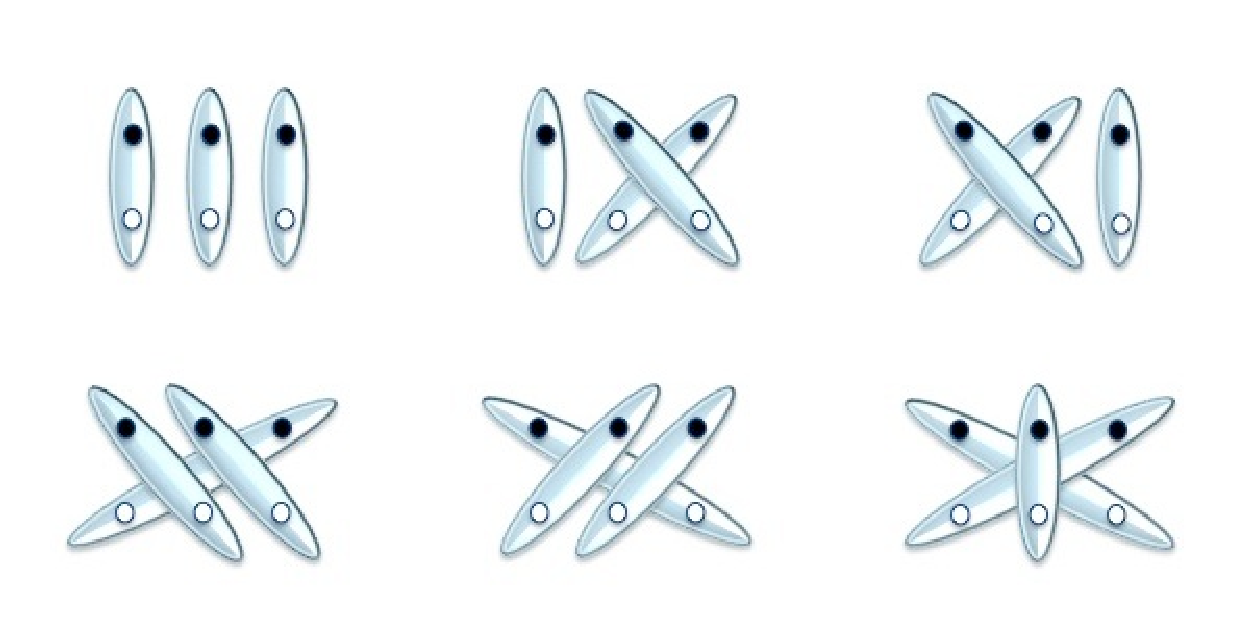
\epsfig{file=figs/fig1.eps,width=80mm}
\caption{Possible singlet coverings for two sublattices, and 3 spins per sublattice.} 
\label{fig:VB1}
\end{figure}
\end{centering}

Therefore, this entanglement persists at infinite distance. If we consider a system with periodic boundary conditions, it is to expect that eventually all spins from one chain will interact with all the spins on the second chain. In a one dimensional system, they cannot hop past each other, but in a chain with periodic boundary conditions, they can wind around the boundaries and come from the other side. Therefore, we will have a superposition of singlets that connect all possible pairs of spins on both chains, and at all distances, with the same amplitude. In order to describe this wave-function it is useful to resort to a valence bond(VB) picture \cite{Pauling1933,Oguchi1989,Beach2006,Tang2011}. Let us assume that each chain corresponds to a sublattice. Then, our wave-function is the equal superposition of all possible valence-bond coverings connecting the two sublattices, as shown in Figure \ref{fig:VB1} for the particular case of three electrons per chain.

In order to prove that our guess accurately describes the physics, we have numerically computed the overlap between the exact ground-state and the variational ansatz on small systems with periodic boundary conditions. We assumed $S^z_{Total}=0$ and taken the number of particles not a multiple of $2$, to avoid degeneracies. We show the results in Figure \ref{fig:ladder}(a), for different values of $J'$. The overlap is $1$ within numerical precision for a range of small values of $J'$. As $J'$ increases, we observe how this overlap becomes smaller, but still remains higher than $0.9$ for $J' < 0.1$. This range depends only on the number of conduction electrons $N$, and tends to get smaller as the $N$ increases. 
%We also show for comparison the overlap with the ansatz for the strong coupling limit, described by a chain of non-interacting hard-core singlets. Notice that this limit both the spin and charge are entangled into Cooper-like pairs, {\it i.e.} excitations are composite objects of two fermions with opposite spins, and twice the mass of the original particles.



Having shown that the ansatz is a good description of the spin-incoherent regime for $J' \rightarrow 0$, we proceed to derive some straight-forward exact results that can be obtained using the variational form of the wave function. For a start, the entanglement between chains originates from the spin, and the charge does not contribute to it. One might feel inclined to think that spins are in a maximally entangled state. However, we should not forget that the VB basis is overcomplete, and in fact, the entanglement entropy is not $S=N\log2$, as one might expect for a state with $N$ singlets. Using the exact wave-function it is relatively easy to obtain a closed expression for $S$. For calculating the entanglement entropy between the conduction electrons in one chain and the electrons in the bath, which here is the second chain, we squeeze the chains by removing all the unoccupied sites, reducing the configuration space to a spin problem with no charge, as illustrated in Figure \ref{fig:VB1}. In this cartoon, the black dots and white dots will be referred to as A and B sub-lattices. Each sublattice will have $N$ sites, instead of $L$, where $N$ is the number of electrons in each chain. Both sublattices have the same number of sites, and the ground-state is represented by all possible VB coverings connecting the two.  
Instead of using the overcomplete  VB basis for the calculation, we will work in the space of spin configurations. In this basis, the states can be classified by the number $N_\downarrow$ of down spins in sublattice A. Since the total spin projection $S^z$ is conserved, this also fixes the number of down spins on sublattice B. The coefficient in front of each configuration is then given by
\begin{equation}
g(N,N_\downarrow)=N_{\downarrow} !(N-N_{\downarrow})! \times (-1)^{N_{\downarrow}},
\label{deg}
\end{equation}
which counts the number of times each of them is repeated in the ground-state, times a sign arising from the singlets (we have ignored the normalization for the time being).

\begin{centering}
\begin{figure}
\epsfig{file=figs/fig2.eps,width=50mm,angle=-90}
\caption{Exact diagonalization results for small ladders of length $L$, and $N$ electrons per chain: (a) overlap with variational wave-function, and (b) entanglement entropy between chains, normalized by the exact value for $J'\rightarrow0$.} 
\label{fig:ladder}
\end{figure}
\end{centering}

The Von Neumann entanglement entropy $S$ is defined as
\begin{equation}
S_\mathrm{A}=-\mathrm{Tr}\left( \rho_\mathrm{A}\log{\rho_\mathrm{A}} \right),
\label{S_A}
\end{equation}
where $\rho_\mathrm{A}$ is the reduced density matrix for sublattice A, obtained by tracing over the states on sublattice B.
It is easy to see that $\rho_\mathrm{A}$ can be separated into blocks, each labeled by $N_\downarrow$. Since $N_\downarrow$ can assume values $N_\downarrow=0,\cdots,N$, the number of such blocks is $N+1$. The linear dimension for each block is given by the number of possible arrangements of $N_\downarrow$ spins in $N$ sites:
\[
d(N,N_\downarrow)=\frac{N!}{N_\downarrow ! (N-N_\downarrow)!}.
\]

It is easy to see that, since all configurations with fixed $N_\downarrow$ will appear with the same coefficient, each block will have all matrix elements equal to $\rho_\mathrm{A}(N,N_\downarrow)_{i,j}=d(N,N_\downarrow) g^2(N,N_\downarrow)$:
\begin{equation}
\rho_\mathrm{A}(N,N_\downarrow)=d(N,N_\downarrow) g^2(N,N_\downarrow)
\left(
\begin{array}{cccc}
1 & 1 & \cdots & 1 \\
1 & 1 & \cdots & 1 \\
\vdots & \vdots & \ddots & \vdots \\
1 & 1 & \cdots & 1
\end{array}
\right)
\end{equation}

This matrix has only a single non-zero eigenvalue $w(N,N_\downarrow)=d^2(N,N_\downarrow)g^2(N,N_\downarrow)=(N!)^2$, the same for all blocks.
Finally, the full matrix has to be normalized such that $\mathrm{Tr}(\rho_\mathrm{A})=1$. Therefore, we obtain $N+1$ blocks, each with a single non-zero eigenvalue $w=1/(N+1)$. Hence, the entanglement entropy (\ref{S_A}) is given by:
\[
S_\mathrm{A}=\log{(N+1)},
\]
which is our final result. 

This expression is equivalent to two spins $S=N/2$ in a maximally entangled state, where each spin is obtained by the addition of the $N$ spins $1/2$ of each sublattice, instead of $N$ spins $1/2$ in a maximally entangled state. 
This analogy can be made rigorous by observing that the spin wave-function is the ground-state of the Hamiltonian:
\[
H_\mathrm{AB}=\sum_{i,j} \vec{s}_{i,\mathrm{A}}\cdot \vec{s}_{j,\mathrm{B}} = \vec{S}_\mathrm{A} \cdot \vec{S}_\mathrm{B},
\]
with $\vec{S}_\mathrm{A} = \sum_i \vec{s}_{i,\mathrm{A}}$, and a similar expression for sublattice B. The ground state is a singlet of two spins $S=N/2$, a maximally entangled state. Notice that this is not the actual spin Hamiltonian for the coupled $t-J$ chains, since the spectra are different. Now we can make use of this solution to calculate the spin-spin correlations. The Hamiltonian can be re-written as:
\[
H_\mathrm{AB}=\frac{1}{2}\left[(\vec{S}_\mathrm{A}+\vec{S}_\mathrm{B})^2-\vec{S}_\mathrm{A}^2-\vec{S}_\mathrm{B}^2 \right].
\]

From this expression, we obtain the ground-state energy:
\[
\langle H_\mathrm{AB}\rangle = \sum_{i,j} \langle \vec{s}_{i,\mathrm{A}}\cdot \vec{s}_{j,\mathrm{B}}\rangle = -\frac{N}{2}\left(\frac{N}{2}+1\right).
\]

Since all the correlators should be equal, we find:
\[
\langle \vec{s}_{i,\mathrm{A}}\cdot \vec{s}_{j,\mathrm{B}}\rangle = \frac{1}{N^2} \langle H_\mathrm{AB}\rangle = -\frac{1}{4}-\frac{1}{2N}.
\]

In order to calculate the correlations in the actual $t-J$ ladder we need to include the charge contribution:
\[
\langle \vec{s}_{i,1} \cdot \vec{s}_{j,2} \rangle = (-\frac{1}{4}-\frac{1}{2N})\langle n_{i,1} n_{j,2} \rangle = (-\frac{1}{4}-\frac{1}{2N})\left(\frac{N}{L}\right)^2,
\]
which indicates that the correlations saturate in the thermodynamic limit.

In Figure \ref{fig:ladder}(b) we show the entanglement entropy, normalized by the exact value for $J'=0$. Same as the overlap, the expression holds for a range of $J'$, and $S$ increases as the charge becomes also entangled with the spin. 

It is enlightening to calculate the momentum distribution function (MDF) for the fermions:
\begin{equation}
n(k) = (1/L)\sum_{l,\sigma} \mbox{exp}(ikl)\langle c^\dagger_{1,\sigma}c_{l,\sigma}\rangle.
\label{nk}
\end{equation}

In order to estimate this quantity, we follow Ref.\onlinecite{Penc1997} and break the fermionic operators $c^\dagger_{i,\sigma}$ and $c_{i,\sigma}$ into a spinless fermionic operators $f^\dagger_i$,$f_i$ acting on the (spinless) charge part of the wave-function, and new operators $Z^\dagger_{i,\sigma}$ and $Z_{i,\sigma}$ acting on the spin part of the wave-function. These spin operators have a very peculiar behavior: $Z^\dagger_{i,\sigma}$ inserts a spin $\sigma$ to the spin chain after skipping the first $i-1$ spins and makes it $N+1$ sites long, while $Z_{i,\sigma}$ has the opposite effect, shortening the chain. For instance, for the first site of the chain, we have:
\begin{equation}
c^\dagger_{1,\sigma}=Z^\dagger_{1\sigma}f^\dagger_1 \mspace{20mu} and \mspace{20mu} c_{1,\sigma}=Z_{1\sigma}f_1.
\end{equation}

The generic expression for the operators can become more complicated, since to act with the $Z$ operators on the spin chain, we need to count the number of charges on the spinless fermion chain. We refer the reader to Refs.\onlinecite{Sorella1991,Pruschke1991,Penc1997,Penc1997b} for details. The action of the operators $c^\dagger_{1,\sigma}c_{l,\sigma}$ is to move a fermion from site $l$ to site $1$. If there are no particles in between, the spin wave-function will remain unchanged. If there is one or more particles in between, it is quite easy to realize that since the spin wave-function is the equal sum of all singlet coverings, it will also remain so after moving one of the ends of a singlet across any number of sites. Therefore, the momentum distribution function reduces to 
\begin{equation}
n(k) = (1/L)\sum_{l,\sigma} \mbox{exp}(ikl)\langle f^\dagger_{1}f_{l}\rangle,
\label{nkb}
\end{equation}
which is nothing else but the MDF for spinless fermions. Since the charge wave-function is that of non-interacting particles, we find that the excitations are free spinless fermions with quasi-particle weight $z=1$, and Fermi momentum $2k_F$. 
%This is a remarkable result, since the uncoupled systems are Luttinger liquids, with zero quasi-particle weight, and no coherent single-particle excitations! 
In Figure \ref{fig:mdf}(a) we show the MDF calculated for large systems using the density matrix renormalization group (DMRG) method \cite{White1992,White1993}, indicating that the quasi-particle weight may remain finite for a range of $J'$. We have to concede that since the calculations are on finite-systems with $L=30$ sites and $N=15$ electrons per chain, we cannot argue with full certainty that the discontinuity at $k=2k_F$ is not actually a singularity, and this remains an interesting problem to pursue. 

\subsubsection {$t-J$ Kondo Chains}

We consider a Kondo chain in which the conduction electrons strongly interact, and are described by Hamiltonian (\ref{H_t-J}). At the same time, the electrons are antiferromagnetically coupled to localized impurities via an exchange $J_K$:
\begin{equation}
H_K=J_K \sum_{i=1}^L \vec{s}_i \cdot \vec{S}_{i},
\label{fullH}
\end{equation}
where  $\vec{s}_i$ describes the conduction spins  and $\vec{S}_i$ the localized spins. It is easy to see that this is equivalent to the two coupled chains, in which one of them is at half-filling. Curiously, this model has not received much attention in the literature. It has been shown that in the limit of $J\rightarrow0$, any infinitesimal $J_K$ will yield a ferromagnetic ground-state\cite{Yanagisawa1994}, in which the localized impurities are underscreened: the $N$ conduction spins will screen $N$ impurity spins, and the remaining ``unpaired'' impurities will be in a ferromagnetic state with maximum spin $S_{Total}=(L-N)/2$. Notice that this means that the paramagnetic state with a large Fermi surface is totally suppressed in this regime. 

\begin{centering}
\begin{figure} [!h]
\epsfig{file=figs/fig4.eps,width=80mm}
\caption{Possible singlet coverings for two sublattices with unequal number of sites, and an excess up-spin.} 
\label{fig:VB2}
\end{figure}
\end{centering}

This state will be a multiplet, and for convenience we focus on the configuration with projection $S^z_{Total}=S_{Total}$. Following a similar reasoning as in the previous part, we argue that the $N$ conduction electrons will form the same VB state as the one described before, while the unpaired impurities will all point in the same direction. The polarized spins can sit on any site of the lattice with equal probability. Therefore, our ansatz can be written as:
\begin{equation}
|\mathrm{g.s.}\rangle=|\phi\rangle \otimes |S\rangle \otimes |\sigma\rangle,
\label{gs4}
\end{equation}
where $|S\rangle$ is the VB wave function, and $|\sigma\rangle$ indicates the positions of the unpaired polarized spins:
\[
|\sigma\rangle = \sum_{x} |x\rangle,
\]

This wave-function is the sum with equal amplitude of all the configurations $|x\rangle$ of $L-N$ particles in $L$ sites.
Figure \ref{fig:kondo}(a) shows the overlap between the exact and variational ground-states, and we again observe identical behavior as the $t-J$ ladder. 

The VB basis for this problem is overcomplete, and we also have to account for the unpaired polarized spins, as shown schematically in Figure \ref{fig:VB2}. This generalization can be easily carried out\cite{Damle2010}, and it is still straightforward to obtain a closed expression for the entropy, which is slightly different than the one for the coupled chains. The calculation for the $t-J$-Kondo lattice follows identical steps, except that since the B sublattice has $L$ sites, the degeneracy for each sector acquires a slightly more elaborate form:
\[
g(L,N,N_\downarrow)=\dfrac{(N-N_{\downarrow})! (L-N+N_{\downarrow})!}{(L-N)!} \times (-1)^{N_{\downarrow}}.
\]

In this case, the single non-zero eigenvalues for each sector are given by:
\[ 
w(L,N,N_\downarrow)=d(L,N,N_\downarrow)g^2(L,N,N_\downarrow)d_\mathrm{B}(L,N,N_\downarrow),
\]
where
\[
d_\mathrm{B}(L,N,N_\downarrow)=\frac{L!}{(L-N+N_\downarrow)!(N-N_\downarrow)!},
\]
is the number of configurations in the B sublattice, for each configuration of the A sublattice. Since the eigenvalues are different for each sector, the normalization and the entropy are obtained by adding numerically over the $N+1$ blocks. We show results in Figure \ref{fig:kondo}(b), which have strong resemblance with those for the ladder. 

\begin{centering}
\begin{figure}
\epsfig{file=figs/fig5.eps,width=50mm,angle=-90}
\caption{Exact diagonalization results for small $t-J$ Kondo chains of length $L$, and $N$ conduction electrons: (a) overlap with variational wave-function, and (b) entanglement entropy between chains, normalized by the exact value for $J_K\rightarrow0$.} 
\label{fig:kondo}
\end{figure}
\end{centering}



The calculation of the MDF is strictly the same as before and the results are identical for $J_K=J'=0$. Notice however, that unlike the $t-J$ ladder, the MDF for up and down spins will be different, and only the sum of the two will be the same. This is shown in Figure \ref{fig:mdf}(b),(c), and (d). In particular, there is a striking difference between the MDF for the majority up and minority down electrons. The up electrons present a clear discontinuity at the Fermi level, while the down electrons display the behavior of a Luttinger liquid with zero quasi-particle weight. The sum of the two, shown in Figure \ref{fig:mdf}(b) of course hides these interesting features. This resembles the behavior of a Fulde-Ferrell-Larkin-Ovchinnikov (FFLO) polarized paired state in one dimension\cite{Yang2001,Orso2007,Feiguin2007c,Feiguin2009b,Heidrich-Meisner2010,Lutchyn2011,Dalmonte2012}. However, the physics of our problem is quite different, since only the spin entangles, and not the charge. We would rather call this state a ``half-Fermi-liquid'', or ``half-Luttinger-liquid''. Whether these are finite-size artifacts or not, undoubtedly, it is a problem that requires further study.
We point out again that the shift to a larger momentum in the MDF should not be confused with a large Fermi surface, that is a feature of the {\it paramagnetic} phase of the Kondo lattice. 

\begin{centering}
\begin{figure}
\epsfig{file=figs/fig3.eps,width=80mm,angle=-90}
\caption{Momentum distribution function for (a) coupled $t-J$ chains as a function of the inter-chain coupling $J'$, and (b),(c),(d) the Kondo lattice, as a function of the Kondo coupling $J_K$. The two lower panels show the results for different spin orientations. Calculations were done with DMRG for a system of size $L=30$ and $N=15$ conduction electrons, and periodic boundary conditions.} 
\label{fig:mdf}
\end{figure}
\end{centering}

Our DMRG results indicate that the variational wave functions describe the physics of the problem in a range of $J'$ and $J_K$. In this regime, the charge and the spin can be considered to a good extent as separate degrees of freedom with independent dynamics: the charge can be described as non-interacting spinless fermions in the ground-state, while the spin is entangled into a VB-like state where all valence bond coverings have the same weight. The inter-chain coupling $J'$ and the Kondo interaction $J_K$ parametrize an effective {\it spin} temperature. If we trace over the bath, the spins of an isolated chain will be in equilibrium at a certain ``quasi-spin temperature''. This spin temperature is not infinite, since we have proven that the spin is not maximally entangled. However, this state seems to correspond to a fine-tuned point in which excitations can be described as free spinless fermions.

The introduced wave-functions establish a framework to study spin-incoherent behavior in systems with spin-charge separation. Normally considered a finite-temperature scenario, this physics can also be realized at zero temperature, once the system is coupled to external spin degrees of freedom. It is not restricted to the models used in this work for illustration, but the theory can be easily extended and generalized to other cases, such as an arbitrary number of coupled $t-J$ chains, for instance \cite{Anderson1990,Putikka1994}. 

We point out that even though our study applies to systems with periodic boundary conditions, same ideas apply to problems with open boundary conditions. In that case, we expect the VB wave-function to be quite different, with only the first kind of configurations shown in Figure \ref{fig:VB1} carrying most of the weight, and a consequent entanglement entropy $S=N\log{2}$ corresponding to infinite effective spin temperature \cite{Feiguin2011}. 

Contrary to other problems studied with VB-type variational wave-functions \cite{Sandvik2012}, the accuracy of our ansatze seems to depend primarily on the number of particles $N$, and not the size of the chains $L$, which may suggest that our description will still be valid for large systems, as long as the density is sufficiently small. Yet, our DMRG results a quarter-filling still display the same physics. In any case, one has to keep in mind that our considerations are strictly valid in the limit $J',J_K\rightarrow 0$.
\pagebreak
\section {Spectral signatures of spin-charge separation}

As seen above, the factorized wave function contains already all the ingredients to qualitativelye, and even quantitatively, understand the phenomenon of spin-charge separation. We are particularly interested in the effects of temperature on the spectral function of the Hubbard model in the large $U$ limit.
In this limit, the spinon band is non-dispersive, and an infinitesimally small temperature will drive them effectively incoherent, leading to the SILL paradigm.

This crossover from spin-coherent to spin-incoherent is characterized by a transfer of spectral weight. Remarkably, the photoemission spectrum of the SILL can be understood by assuming that after the spin is thermalized, the charge becomes spinless, with a shift of the Fermi momentum from $k_F$ to $2k_F$ \cite{Feiguin2011}. 
Clearly, this behavior defies our intuition, since the excitation spectrum of the problem is completely determined by the Hamiltonian, at finite temperature (and in the absence of phase transitions) we only expect a redistribution of spectral weight. This paradox can be reconciled in the context of spin-charge separation. If we assume that spin and charge degrees of freedom are completely decoupled, the single-particle spectral function of the electrons can be understood as the convolution of the charge and spin dynamical correlation functions. 
%The  charge will remain pretty much unaffected by temperature, while the spectrum of the spin will undergo a dramatic redistribution of spectral weight.  

In this chapter, we use Ogata and Shiba's factorized wave function\cite{Ogata1990}, complemented by t-DMRG calculations at finite spin temperature, to obtain the spectral function of strongly interacting Hubbard chains ($U\rightarrow\infty$) in the crossover between spin-coherent and spin-incoherent regimes. 

\subsection{Method}
In order to calculate the spectral functions, we follow the formalism developed in Refs.\onlinecite{Sorella1991,Pruschke1991,Penc1997b}, described in great detail in Ref.\onlinecite{Penc1997}. We sketch the main ideas, avoiding technicalitites and directing the reader to the aforementioned references. In the $U\rightarrow\infty$ limit, using Bethe ansatz, Ogata and Shiba demonstrated that the exact solution can be factorized and split into two parts:
\begin{equation}
|\psi^{N,GS}_L\rangle= | \phi\rangle\otimes | \chi\rangle,
\label{gs}
\end{equation}
where $|\phi\rangle$ describes the charge and is comprised by spinless fermionic degrees of freedom, and $|\chi\rangle$ is consistent with a ``squeezed'' chain of $N$ spins, where all the empty sites have been removed. $|\phi\rangle$ is simply the ground-state of a one-dimensional tight-binding chain of $N$ non-interacting spinless fermions on a lattice with $L$ sites. The factorization applies also to excited states as:
\begin{equation}
\label{ex_state}
|\mathrm{\psi(P)}\rangle= | \phi^N_{L,Q}(P,I)\rangle \otimes | \chi^{N_\downarrow}_N(Q,M)\rangle,
\end{equation} 
where $I$ labels a combination of $N$ momenta $k_i L = 2 \pi i + Q$ ($i=-L/2,-L/2+1,\cdots,L/2-1$) that are compatible with the total fermionic momentum $P$. The index $M$ labels all possible configurations of momenta compatible with the total momentum of the spin wave function $Q=2\pi j/N$, with $j=0,1,\cdots,N-1$.
The fermionic part stays coupled to the spin part only by a phase $Q$ imposed to the boundaries, resulting in twisted boundary conditions for the fermions, which ensures momentum conservation for the original problem. This phase is $Q=\pi$ for the ground-state $|\psi^{N,GS}_L\rangle$, and we would fill up the Fermi sea minimizing the energy by choosing the combination of momenta $\{-\frac{N}{2},-\frac{N}{2}+1,...,\frac{N}{2}-1\}$ \cite{Penc1997b}.

The dynamics of the spinless fermions is governed by a tight-binding Hamiltonian, with an energy dispersion $\epsilon(k)=-2t\cos(k)$, while the spin degrees of freedom are in principle non-interacting. For finite but large $U\gg t$, the physics of the spins can be approximated by that of a Heisenberg spin chain, with $J =4nt^2[1-\sin{(2\pi n)}/(2\pi n)]/U$, where $n=N/L$ is the density \cite{Penc1997,Xiang}.

In order to calculate the Green's functions for the electrons, we start by noticing that destroying an electron in the original Hubbard chain would translate into the anihilation of a fermion in the charge wave function, and a spin in the spin chain (and the opposite effect for the creation operator). This is achieved by introducing new operators such that $c_{i_\sigma}=f_iZ_{l(i),\sigma}$, where $f_i$ is a fermionic anihilation operator without spin, acting at position $i$ on the fermionic wave function, and $Z_{l(i),\sigma}$ removes a spin $\sigma$ at position $l(i)$ in the spin chain. The operator $Z$ has a peculiar behavior, since it destroys the spin and the site itself, making the spin chain $N-1$ sites long. The index function $l(i)$ indicates the position of the spin that belongs to site $i$ of the original chain, after squeezing the wave function and removing all the holes. The simplest form of the $c_{i_\sigma}$ operator is for the first site:
\begin{equation}
c_{0,\sigma} = f_0 Z_{0,\sigma}.
\label{c_}
\end{equation}

The zero-temperature one-particle spectral function is obtained from the imaginary part of the Green's function. We focus only on the contribution from the occupied levels, corresponding to the photoemission spectrum.  In the Lehmann representation, we write it as
\begin{equation}
B(k,\omega)= \sum_{f,\sigma} |\langle f,N-1 | c_{k,\sigma} | GS,N \rangle |^2 \delta (\omega - E_{GS}^N + E_f ^{N-1}).
\label{B_ck}
\end{equation}

Here $c_{k,\sigma}$ destroys an electron with momentum $k$ and spin $\sigma$, $f$ is the final state with $N-1$ particles and $N$ is the total number of electrons. In order to use the factorized wave-function in the calculation, and working in the real space for more convenience, re-writing this expression as
\begin{eqnarray}
B(k,\omega) & = & \sum_{f,\sigma} L |\langle f,N-1 | c_{0,\sigma} | GS,N \rangle |^2 \delta (\omega - E_{GS}^N + E_f ^{N-1}) \nonumber \\
& & \delta_{k,P_{GS}^N-P_f^{N-1}} ,
\label{B_c0}
\end{eqnarray}
where we have imposed momentum conservation with the term $\delta_{k,P_{GS}^N-P_f^{N-1}}$ and used the definition $c_{j,{\sigma}}=\frac{1}{\sqrt{L}} \sum_{k'} e^{i k' j} c_{k',\sigma}$.  

By taking advantage of the factorized wave-function, Eq.(\ref{ex_state}), and the separated spin and charge operators, Eq.(\ref{c_}) we get the following expression
%\begin{eqnarray}
%B(k,\omega) &=& \sum_{f,\sigma} L | \{ \langle \phi^{N-1}_{L,Q}(I)| \otimes \langle \chi_{N-1}(Q,M) | \} \mid \ Z_{0,\sigma} f_0 \mid \{ |\phi^{N,GS}_{L,\pi}\rangle \otimes |\chi_N^{GS} \rangle \} |^2 \\ \nonumber
%& & \times \delta (\omega - E_{GS,s}^N -  E_{GS,ch}^N + E_{f,s} ^{N-1} + E_{f,ch} ^{N-1}) \times \delta_{k,P_{GS}^N-P_f^{N-1}}
%\label{B_Zb}
%\end{eqnarray}
\begin{equation}
B(k,\omega)= \sum_{Q,\omega',\sigma} D_{\sigma}(Q,\omega') B_Q(k,\omega-\omega').
\label{B_conv}
\end{equation}

In this expression, $B_Q(k,\omega)$ is determined by the spinless fermion operator $f$ as 
\begin{equation}
B_Q(k,\omega)= L \sum_{I} |\langle \phi^{N-1}_{L,Q}(I) | f_0 | \phi^{N,GS}_{L,\pi}\rangle | ^2 \delta (\omega - E_{GS,ch}^N + E_{f,ch} ^{N-1}) \times \delta_{k,P_{GS}^N-P_f^{N-1}},
\label{B_Q}
\end{equation}
where the the fermionic energies are obtained from the tight-binding dispersion.
$D_{\sigma}(Q,\omega)$ is defined by the action of the spin operators $Z$: 
\begin{equation}
D_{\sigma}(Q,\omega)= \sum_{M} |\langle \chi_{N-1}(Q,M) |  {Z}_{0,\sigma} | \chi_N^{GS} \rangle | ^2 \delta (\omega - E_{GS,s}^N + E_{f,s} ^{N-1}).
\label{D_sigma_Q}
\end{equation}

To calculate the $D_{\sigma}(Q,\omega)$ we need to solve the spin-$\frac{1}{2}$ Heisenberg Hamiltonian to obtain the energies and the wave-functions for $N$ and $N-1$ sites. In the $U\rightarrow \infty$ and $J \rightarrow 0$ limit the excitation spectrum collapses and $D_{\sigma}(Q,\omega)=D_{\sigma}(Q)\delta(\omega)$. The function  $D(Q)$ can be derived by using the spin transfer function $\omega_{j' \rightarrow j,\sigma}$ defined by Ogata and Shiba \cite{Ogata1990,Ogata1991}, and by Sorella and Parola \cite{Sorella1991}. This function gives the amplitude of moving the spin $\sigma$ from site $j'$, to $j$. For $j'=0$ it is given by
\begin{equation}
        \omega_{0 \rightarrow j,\sigma} = \langle \chi_N^{GS} \mid P_{j,j-1} \dotsb  P_{0,1} \delta_{\sigma,S_0^Z} \mid \chi_N^{GS} \rangle,
\label{omega}
\end{equation}
where we introduced the permutation operator $P_{j,j-1} = 2 \vec{S}_j \cdot \vec{S}_{j-1} + \frac{1}{2}$, that exchanges the spins at sites $j$ and $j-1$. Using this spin transfer function we get
\begin{equation}
        D_{\sigma}(Q) = \frac{1}{N-1} \sum_{j=0}^{N-2} e^{i (Q+\pi)j} \omega_{0 \rightarrow j,\sigma}.
\label{D_Q}
\end{equation}

For finite but small $J$ one can use the approximation \cite{Penc1997b}

\begin{equation}
D_{\sigma}(Q,\omega) = D_{\sigma}(Q) \delta (\omega - E_s + \epsilon_Q),
\label{cloizeaux}
\end{equation}
%
where $\epsilon_Q = \frac{\pi}{2} J |\sin(Q-\pi/2)|$ is the des Cloizeaux-Pearson dispersion, and $E_s = - J \ln 2$ is the ground state energy, which are obtained from the exact Bethe ansatz solution for the Heisenberg chain \cite{Cloizeaux}.



\subsection {Generalization to finite temperatures}

The expression (\ref{D_Q}) can be generalized to finite {\it spin temperatures} $\beta_\sigma=1/T_\sigma$ as
\begin{equation}
\label{D_Q_beta}
D_{\sigma}(Q,\beta) = \frac{1}{N-1} \frac{1}{Z_s} \sum_{j=0,M_Q}^{N-2} \omega_{0 \rightarrow j,\sigma} e^{i (Q+\pi)j} e^{- \beta E_{M_Q,s}},
\end{equation}
where $Z_s$ is the spin partition function.
In order to calculate  this quantity numerically, we resort to t-DMRG calculations at finite temperature. The problem reduces to evaluating the thermal average of $\omega_{0 \rightarrow j,\sigma}$, described by Eq.(\ref{omega}), for a one-dimensional Heisenberg chain. The antiferromagnetic exchange is set to $J=1$, and the spin temperature $\beta_\sigma$ is defined in units of $J$. For the final calculation, we approximate $D(Q,\omega,\beta_\sigma)$ using the prescription (\ref{cloizeaux}). 

\begin{figure}
%\vspace{0.25cm}
\epsfxsize=7cm \centerline{\epsfbox{figs/zk.eps}}
\caption{ 
Correlation function for the spins $D(Q)$ calculated on Heisenberg spin chain ($J=1$), for different temperatures, obtained with the time-dependent DMRG.
}
\label{figure1}
\vspace{0.25cm}
\end{figure}

Since the Heisenberg chain is weakly entangled at high temperatures, $T_\sigma > J$, we are able to simulate systems as large as 300 sites. We point out that the calculation of $\omega_{0 \rightarrow m,\sigma}$ is not that trivial, since it involves building a string of permutations between all pairs of spins between sites $0$ and $m$. To do this, we use a recipe similar to the one used to time-evolve the wave-function in t-DMRG. Since the structure of the DMRG block decimation always leaves two individual single sites in the original spin basis, we apply the permutation operator between these two sites. We propagate the wave function to the next iteration, and apply the next permutation. This builds a chain of permutations as the DMRG algorithm sweeps through the lattice. In order to calculate the quantum mechanical average, we need to use two target states, the original thermal state (or the ground state at $T_\sigma=0$), and the state obtained after applying the permutations. The calculation is done more efficiently if one starts from the first site at the left end of the chain. The application of $P_{1,0}$ yields the first average $\omega_{0\rightarrow 1}$. In the next left-to-right iteration we apply $P_{2,1}$ to the previous state, leading to $\omega_{0\rightarrow 2}$. We can repeat this procedure all the way until we reach the other end of the chain, and a single DMRG sweep yields all the correlations needed to construct $D(Q,\beta_\sigma)$. 




The results for $D(Q,\beta_\sigma)$ are shown in Fig.\ref{figure1}. These are very accurate and for the $\beta_\sigma=0$ limit, they are exact, and can be compared to the expression 
\begin{equation}
\label{D_Q_beta0}
D(Q,\beta_\sigma=0)=\frac{1}{N-1}\frac{3}{10-8\cos{Q}}.
\end{equation}

\begin{figure}
%\vspace{0.25cm}
\epsfxsize=8cm \centerline{\epsfbox{figs/BQ.eps}}
\caption{ 
Spectral function obtained using the factorized wave function, for $J=0.05$, $L=56$ sites, and $N=42$ fermions. The panels correspond to different values of the ``spin temperature'' (see text).  
}
\label{figure2}
\vspace{0.25cm}
\end{figure}

As the temperature decreases the peak in $Q=0$ shifts toward $Q=\pi/2$, as expected for an antiferromagnetic spin chain. At very low temperatures the correlation function develops a singularity at $Q$, which creates serious finite-size effects in our results. We therefore restrict our simulations to values of $\beta_\sigma$ that we can trust.



In Fig.\ref{figure2} we show the results for the electronic spectral function after the convolution, using the data for $D(Q)$ obtained from the DMRG calculation. We chose the value of $J=0.05$ to compare with the results from Ref.\cite{Feiguin2009d}. We observe identical behavior, the spectral weight shifting in momentum, with the minimum of the dispersion moving from $k=0$ at infinite spin temperature to $k=2k_F$ at zero temperature. 

\subsection {Spin-incoherent behavior}

In the regime studied here, $J/t \rightarrow 0$, a small temperature effortlessly excites the spins while the charge remains on its ground-state resulting spinons become totally incoherent, effectively at infinite temperature. At the fillings we considered the system is gapless and follows a Lutinger Liquid theory. Moreover, this incoherency in spin behavior makes it a SILL at low temperatures. This regime is characterized by universal properties in the spectral functions, causing a spectral weight transfer sensitive to the spin temperature.

This transfer of spectral weight represents a crossover from spin-coherent to spin-incoherent regime, equivalently from LL to SILL. The momentum-resolved photoemission spectrum shown in Fig. \ref{figure2} reveals a drastic change of behavior in the spectral function once the temperature is moved from zero to infinity. At infinite temperature we see a noninteracting band which refers to the spinless fermions following a $-2 t cos(k)$ dispersion (of course here we are only showing the photoemission part of the spectrum). Lowering the temperature the band starts to widen until we see a redistribution of the peak in the $k$ direction, where it splits into two seperate peaks moving from $k=0$ towards $k= \pm k_F$. The two-peaked regime is in the agreement with the scattering of holons with the non-dispersive spinons present in the spin-incoherent regime. At the temperatures in the order of $J$ we see this crossover from spin-coherent to incoherent regime, where qualitatively in a good agreement with experiments in nanowires \cite{Steinberg2006}. 

The ``spin-incoherent'' ground state will have the same qualitative features as the SILL at finite temperature as discussed in chapter II. In the t-J ladder and t-J Kondo examples the spin temperature is govenred by the coupling between the spin bath and we see that for the regime of parameters which were considered, a small coupling $J'$ between the chains results a spin-charge factorization. Spins of the chain can be driven incoherent by this interaction, while the charge remains on the ground state. This physics is completely analogous to the SILL physics at finite temperature. 


%\subsubsection {Spin-Incoherent behavior in the ground-state of model Hamiltonians}




\pagebreak
\section {Phonons}

In the past two decades, we have witnessed a tremendous
improvement in the energy and the momentum resolution of the
angle-resolved photoemission spectroscopy (ARPES), which is one of
the most powerful experimental tools for investigating strongly
correlated materials as we saw in the previous chapters. In particular, recent ARPES spectra of
high-T$_{C}$ cuprates\cite{Lanzara1,Lanzara2}, alkali-doped
fullerides\cite{Gunnarsson}, and manganites\cite{Lanzara3}, have
shown that the interplay of electron-electron (e-e) and
electron-phonon (e-ph) interactions has an important role in the
qualitative and quantitative understanding of the experimental
results. Other examples of materials that show evidence of both
strong e-ph and e-e interactions are the recently discovered
aromatic superconductors\cite{Kubozono,Kosugi,Kato,Subedi,Nomura}.
It is believed that in these compounds the phonon frequency, e-e
and e-ph interaction energy scales are all comparable to the
electron bandwidth, a regime of parameters that represents a
challenge for a theoretical understanding of experiments.

When considering systems at low dimensions, the situation is even
more complicated.
%In one dimension (1-D), strong correlations induce the
%fractionalization of the low-energy excitations, which decouple
%into spin (spinons) and charge (holons) excitations that move at
%different velocities and at different energy
%scales
In one dimension (1-D) due to the strong correlations, the
low-energy states separate into spin (spinon) and charge (holon)
excitations that move with different velocities and are at
different energy scales \cite{Gogolin2004,GiamarchiBook,Deshpande}.
Spin-charge separation has been observed experimentally in
semiconductor quantum wires\cite{Auslander}, organic
conductors\cite{Lorenz}, carbon nanotubes\cite{Bockrath}, and
quantum chains on semiconductor surfaces\cite{Blumenstein}. 
More recently, SCS has been
observed in photoemission experiments on the quasi-1D cuprate
$SrCuO_{2}$\cite{Kim} and in the organic conductor
TTF-TCNQ\cite{Sing}.

The behavior of the photoemission spectrum of these type of
materials, in which it is believed to have a strong interaction
with the lattice degrees of freedom, is not entirely understood.
In particular, one expects that the interplay of e-e and e-ph
interactions have a profound effect on SCS.

%not much of is known about the
%changes/signatures .
%For instance, the role of e-ph interaction in the interpretation
%of unexpected spectral features such as kinks, 'waterfalls' or the
%high energy anomaly in cuprates, is still under debate. It is
%therefore of paramount importance to study spectral properties in
%the strong coupling regime for both e-e and e-ph interactions, and
%in particular the non-adiabatic limit where the lattice response is
%not slower in comparison to the velocities of the charge and spin
%excitations of the correlated electron system.
The basic lattice model used to describe e-e and e-ph interactions
in 1D is the Hubbard-Holstein (HH) Hamiltonian, which incorporates
nearest-neighbor hopping, an on-site Coulomb repulsion and a
linear coupling between the charge density and the lattice
deformation of a dispersion-less phonon mode. Within this model,
the effect of e-ph interaction on SCS has been studied by
Ref.\onlinecite{Tohyama} and \onlinecite{Lin}. In the first paper,
the authors use dynamical density matrix renormalization group
(D-DMRG) and assess the robustness of SCS against e-ph coupling,
interpreting the spectral function as a superposition spectra of
spinless fermions. In the second paper, the authors use cluster
perturbation theory (CPT) and an optimized phonon approach
concluding that the finiteness of the phonon frequency suppresses
SCS. Both papers focused their attention on half-filling,
considering the regime where the phonon frequency is much smaller
than the electronic bandwidth.
%In this paper, we consider a different regime of parameters,
%considering the on-site Coulomb repulsion as the largest energy
%scale in the problem, a strong e-ph interaction and a phonon
%frequency large as half of the electronic band width.
In contrast to these previous studies, we calculate the spectral
function (Photoemission Spectrum, PES) of the HH model in
1-D away from half-filling, developing a controlled
semi-analytical approach valid in the presence of infinitely large
Coulomb repulsion, a strong e-ph interaction and a phonon
frequency as large as half of the electronic bandwidth. In this
approach, we approximate the ground state as a product of the
Ogata-Shiba wave-function\cite{Ogata1990} resulting from the
$U\rightarrow\infty$ Hubbard model and a noninteracting phonon
wave-function. We then compare the results of our semi-analytical
method with those calculated using the time-dependent DMRG
(t-DMRG).
%t-DMRG is an approximation-free numerical technique for
%1-D quantum lattice models, that we apply in the presence of
%phononic degrees of freedom.
In this case, we observe that the e-ph interaction induces a
reduction of the spinon and holon band amplitudes, from weak up to
intermediate e-ph coupling. Eventually, in the strong e-ph
coupling regime, one observes replicas of the spinon and holon
bands separated from the main band by an energy difference
approximately equal to the phonon frequency. The same qualitative
behavior is reproduced by our semi-analytical calculation. In
particular, away from the intermediate e-ph coupling regime, we
obtain a close agreement with t-DMRG results. Phonon degrees of
freedom couple with the charge degrees of freedom and the spinon
is left unaffected in a good approximation. The best agreement is
obtained once the phonon frequency is in the same energy scale of
the charge bandwidth. This rises to having replicas of the
spectrum at intervals of energy proportional to the phonon
frequency.

 %The results agree with the simple interpretation that,
%being the phonon frequency energy scale as large as the electronic
%bandwidth, phonons couple only with the charge degrees of freedom
%giving rise to replicas of the spectrum at intervals of energy
%proportional the the phonon frequency.

%When e-e interactions is sufficiently large, the energy scale of
%the spin excitations is much smaller than the energy scale of the
%charge excitations. In presence of e-ph interactions, one naively
%expects that, when the phonon frequency energy scale is large as
%the electronic bandwidth, phonons couple only with the charge
%excitations....
In the following section we introduce a
semi-analytical method for calculating the spectral function of
the HH model and discuss the validity of the approximations used.

%\section{SEMI-ANALYTICAL METHOD FOR CALCULATING THE SPECTRAL FUNCTION OF THE HUBBARD-HOLSTEIN MODEL IN 1D}

%We would like to consider the effects of phonons on the spectral
%function. Adding the phonon interaction to the problem makes is
%extremely complicated and somehow impossible to be solved
%analytically, because of this fact we will try to tackle this
%problem in a semi-analytical approach and do some parts of the
%calculation by the means of computing. 

\subsection {The Hubbard-Holstein model}
We start with the
Hubbard-Holstein model, which describes Einstein phonons
locally coupled to electrons described by the Hubbard
Hamiltonian. The HH Hamiltonian can be written in the general form
\begin{equation}
 \label{HH}
H=-t \sum\limits_{<i,j>, \sigma}(c^\dagger_{i,\sigma}
c_{j,\sigma} + h.c.) + U \sum\limits_{i} n_{i,\sigma}
n_{i,\bar{\sigma}} + \omega_0 \sum\limits_i a^\dagger_i a_i + g \omega_0
\sum\limits_{i, \sigma} n_{i\sigma} (a_i+a^\dagger_i)
\end{equation}
where $t$ is the hopping amplitude, $U$ is the on-site Coulomb repulsion, $\omega_0$ is the phonon frequency, $g$ is the e-ph coupling constant, $c^\dagger_{i,\sigma}$ ($c_{i,\sigma}$) is the standard electron creation
(annihilation) operator with spin ${\sigma}$ on site $i$, $n_{i,\sigma}=c^\dagger_{i,\sigma} c_{i,\sigma}$ is the electronic occupation operator,
and $a^\dagger_i$ ($a_i$) is phonon creation
(annihilation) operator. The units are such that the Planck constant $\hbar=1$, the lattice parameter $a=1$, and all of the energies are in the units of the hopping parameter $t$.  

It is well known that in the presence of e-ph interaction the problem is
extremely complicated and impossible to solve
analytically. Moreover, even by truncating the Hilbert space of the phononic degrees of freedom, solving the problem numerically remains remarkably expensive. In this section we present a semi-analytical method
that allows us to calculate the photoemission part of the spectral function
\begin{equation}
B(k,\omega)=-\frac{1}{\pi} \mathcal{I}mG(k,\omega)  \mspace{30mu} for \mspace{10mu} \omega < \mu,
\label{B_green}
\end{equation}
 where $G(k,\omega)$ is the electronic single particle Green's function, $k$ and $\omega$ are the momentum and energy of the electron, and $\mu$ is the chemical potential.
 We are interested in studying the regime where $U \rightarrow \infty$, in which the electronic double occupancy can be neglected. Our semi-analytical approach consists of variational canonical transformation and is valid in the limit of strong coupling $U >> g^2 \omega_0 > t$, and large phonon frequency $\omega_0 >t$. In this regime, we will show that the model can be described by spin-charge separated polarons. 
 The variational canonical transformation is
\begin{equation}
\label{can_trans} T[f,\Delta] = e^{g \sum\limits_j [n_j f + \Delta](a_j - a^\dagger_j)}
\end{equation}
in which $f$ and $\Delta$ are variational parameters. The quantity $f$ governs the magnitude of the antiadiabatic polaronic effect, while $\Delta$ represents the lattice distortion unaffected by the electrons' position. The transformed Hamiltonian is
\begin{eqnarray}
\label{trans_HH_1}
&&\tilde{H}[f,\Delta]=T^{-1} HT=-t \sum\limits_{<i,j>,
\sigma}(c^\dagger_{i,\sigma} X^\dagger_i X_j c_{j,\sigma} +
h.c.) + (U-2 g^2 f^2 \omega_0) \sum\limits_{i} n_{i,\sigma} n_{i,\bar{\sigma}} \\
&&+ \omega_0 \sum\limits_i a^\dagger_i a_i + L g^2 \omega_0 \Delta^2 + g \omega_0 (1-f) \sum\limits_i n_i (a_i+a^\dagger_i) - g
\omega_0 \Delta \sum\limits_i (a_i+a^\dagger_i)  + \eta \sum\limits_i n_i , \nonumber
\end{eqnarray}
where $L$ is the total number of sites. Here we have defined a phonon operator $X_i = e^{g f (a_i -
a^\dagger_i)}$ and $\eta = g^2 \omega_0 f (f-2) + 2 g^2 \omega_0
(f-1) \Delta$. 
Now we will determine the parameters $f$ and $\Delta$ by using an effective electronic Hamiltonian, $H_{eff}$, which is basically obtained by averaging $\tilde{H}$ on the phononic vacuum, $H_{eff} [f,\Delta] = \langle O_{ph}|\tilde{H}|O_{ph}\rangle$
\begin{equation}\label{Heff_def}
H_{eff} [f,\Delta]=-t e^{-g^2 f^2} \sum\limits_{<i,j>,
\sigma}(c^\dagger_{i,\sigma} c_{j,\sigma} + h.c.)+(U-2 g^2 f^2 \omega_0) \sum\limits_{i} n_{i,\sigma}
n_{i,\bar{\sigma}} + \eta \sum\limits_i n_i  + L g^2 \omega_0 \Delta^2.
\end{equation}
The parameter $\Delta$ is simply obtained by using the Hellmann-Feynman theorem 
\[
\frac {\partial}{\partial \Delta} \langle g.s.|H_{eff}|g.s.\rangle = 0 \Rightarrow
\Delta = (1-f) \frac {N}{L},
\]
where $N$ is the total number of electrons, $N/L$ is the electronic density, and $|g.s. \rangle$ is the ground state of $H_{eff}$. 
Now we are left only with the determination of the parameter $f$, which will be found by solving the Hamiltonian
\begin{equation} \label{Heff_f}
H_{eff} [f]=-t e^{-g^2 f^2} \sum\limits_{<i,j>,
\sigma}(c^\dagger_{i,\sigma} c_{j,\sigma} + h.c.) + (U-2 g^2 f^2 \omega_0) \sum\limits_{i} n_{i,\sigma}
n_{i,\bar{\sigma}} + g^2 \omega_0 (1-f)^2 N^2/L + \eta N,
\end{equation}
by using DMRG and minimizing the ground-state energy of this new Hamiltonian $H_{eff}$ as a function of $f$. For each set of values $U$, $t$, $g$, and $\omega_0$, considered in the original Hamiltonian, we get a $\tilde{f}$. 

In the Figure \ref{fig:f_best_energy}(a), the ground-state energy of $H_{eff}[f]$ as a function of $f$ for two different values of e-ph coupling $g=0.8$ and $g=1.6$, $N/L=0.75$, and $\omega_0=2.0$ is shown.
For $g=1.6$  the value of $\tilde{f}$ obtained is close to $0.8$ meaning that for these sets of parameters the system is near the poloranic anti-adiabatic regime, that ideally is expected to be reached for stronger e-ph coupling and phonon frequency.


\begin{centering}
\begin{figure}
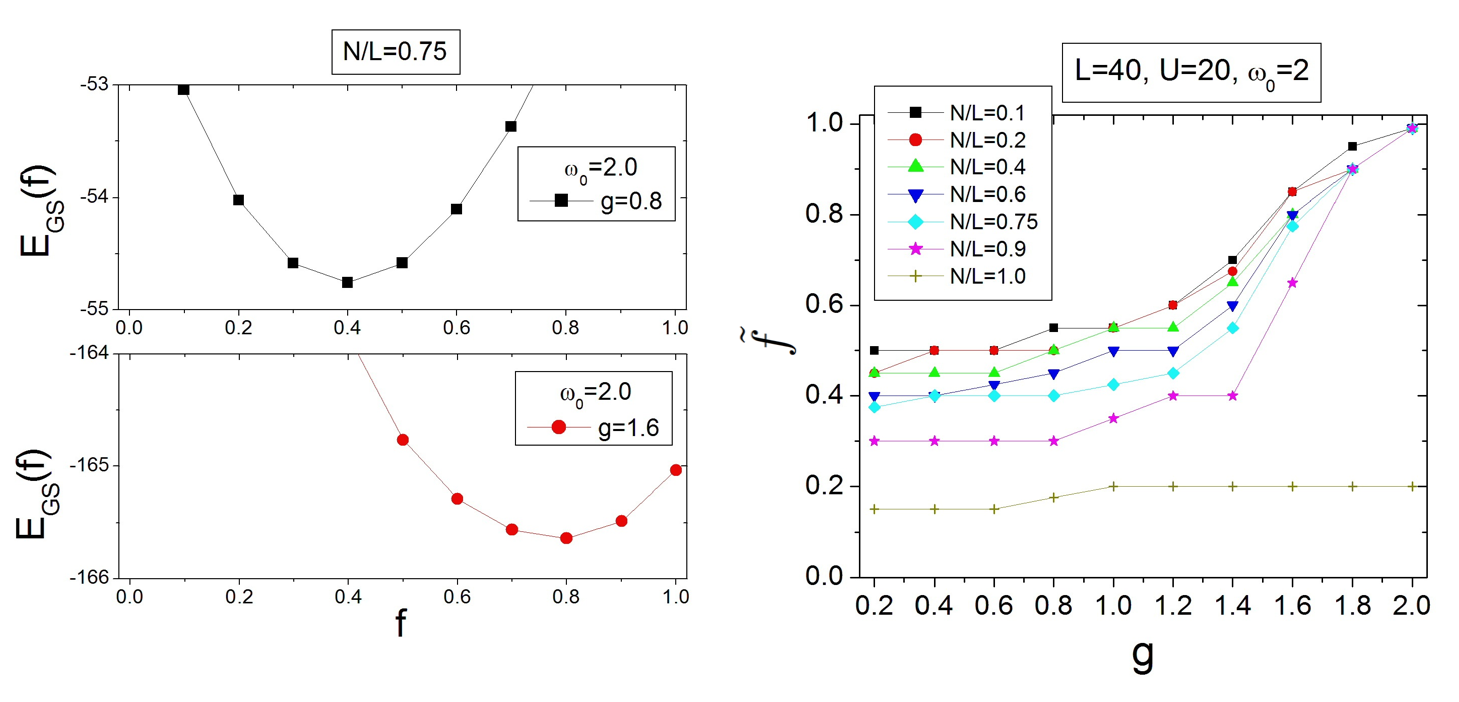
\epsfig{file=figs/EG_f,width=125mm,angle=0}
\caption{(a) The ground-state energy as a function of $f$ in order to get $\tilde{f}$. (b) $\tilde{f}$ as a function of $g$ for different fillings.} 
\label{fig:f_best_energy}
\end{figure}
\end{centering}

In the Figure \ref{fig:f_best_energy}(b) the results of $\tilde{f}$ calculated by DMRG is shown for different values of $g$ and different densities. 
Knowing the $\tilde{f}$ for our problem with the given parameters one can rewrite the original transformed Hamiltonian as
\begin{eqnarray}
\label{Htilde1}
&&\tilde{H}[\tilde{f}]=-t \sum\limits_{<i,j>, \sigma}(c^\dagger_{i,\sigma} X^\dagger_i X_j c_{j,\sigma} + h.c.) + \omega_0 \sum\limits_i a^\dagger_i a_i + (U-2 g^2 \tilde{f}^2 \omega_0) \sum\limits_{i} n_{i,\sigma} n_{i,\bar{\sigma}} \\
&&+ g \omega_0 (1-\tilde{f}) \sum\limits_i n_i (a_i+a^\dagger_i) - g \omega_0 (1-\tilde{f}) \frac{N}{L} \sum\limits_i (a_i+a^\dagger _i)
+ g^2 \omega_0 (1-\tilde{f})^2 \frac {N^2}{L} + \eta N, \nonumber
\end{eqnarray}
with $\eta = g^2 \omega_0 \tilde{f} (\tilde{f}-2) - 2 g^2 \omega_0 (1-\tilde{f})^2 N/L$.


The goal is to use a polaronic variational ansatz by applying a canonical transformation and using the concept of Ogata-Shiba's factorized wave-function to calculate the spectral function. In the end obtained solution by this ansatz will be compared with the results coming from the exact DMRG method. We call it exact since the existing error is in the order of machine precision. One needs to split the Hamiltonian into separated parts that are considered unperturbed and interaction fragments, in order to get a wave-function that is divided into a spinless polaron and a spinfull part
\begin{equation}
\label{Htilde_def} \tilde{H}[\tilde{f}] = \tilde{H}_0 + V,
\end{equation}
where $\tilde{H}_0$ is the unperturbed part, while $V$ is the interaction
\begin{equation}
\label{V_def} 
V = -t \sum\limits_{<i,j>,\sigma}[c^\dagger_{i,\sigma} (X^\dagger_i X_j - e^{-g^2 \tilde{f}^2})
c_{j,\sigma} + h.c.] + g \omega_0 (1-\tilde{f}) \sum\limits_i n_i
(a_i+a^\dagger_i).
\end{equation}

The $\tilde{f}$ provided by acting DMRG on $H_{eff}$, shown in Figure \ref{fig:f_best_energy}(b), is meant to minimize the error produced by neglecting the interaction term $V$ from the Hamiltonian $\tilde{H}[\tilde{f}]$, so we would be able to approach the problem numerically. One can use a perturbation approach and consider the effect of higher orders in perturbation, but here we are only taking the zeroth order into account. Although we are calling the $\tilde{H}_0$ a non-interacting term, it still consists a lot of information about interacting terms in the original Hamiltonian, since most of the parameters of the new problem are renormalized by our technique and we will see the features of an interacting system with a simplified Hamiltonian
\begin{eqnarray}
\label{H0_best}
&&\tilde{H}_0 [\tilde{f}] = \tilde{H} - V = -t e^{-g^2 \tilde{f}^2} \sum\limits_{<i,j>, \sigma}(c^\dagger_{i,\sigma} c_{j,\sigma} + h.c.) +(U-2 g^2 \tilde{f}^2 \omega_0) \sum\limits_{i} n_{i,\sigma} n_{i,\bar{\sigma}} \\
&& + \omega_0 \sum\limits_i a^\dagger_i a_i + \eta N- g \omega_0 (1-\tilde{f}) \frac{N}{L} \sum\limits_i
(a_i+a^\dagger_i) + g^2 \omega_0 (1-\tilde{f})^2 \frac {N^2}{L}.\nonumber
\end{eqnarray}

%%%%%%%%%%%%%%%%%%%%%%%%%%%%%%%%%%%%%%%%%%%%
\subsection {Understanding the spectrum of the HH model, interplay between charge, spin and phonons}

As discussed earlier, the general form of the spectral function that we are trying to calculate follows
\begin{equation}
\label{B_ck}
B(k,\omega)=\sum_{\{n_{ph}\},f,\sigma}|\langle |\{n_{ph}\},f,N-1 | c_{k,\sigma} | g.s.,N \rangle |^2 \delta (\omega - E_{gs}^N + E_f ^{N-1} ),
\end{equation}
where $c_{k,\sigma}$ destroys an electron with momentum $k$ and spin $\sigma$, $N$ is the total number of electrons, $f$ is the final state with $N-1$ particles. $E_f ^{N-1}$ is the total energy of the final state, $|\{n_{ph}\},f,N-1\rangle$, where a generic phonon contriubtion is included, and $E_{gs}^N $ describes the energy of the ground state of the original Hamiltonian (\ref{HH}). Since Einstein phonons carry no momentum we can impose the momentum conservation with the term $\delta_{k,P_{GS}^N-P_f^{N-1}}$, and use the definition $c_{j,{\sigma}}=\frac{1}{\sqrt{L}} \sum_{k'} e^{i k' j} c_{k',\sigma}$, to reduce Eq. (\ref{B_ck}) in a calculation involving only site $0$ in the real space and one phonon mode at that site
\begin{equation}
\label{B_c0}
B(k,\omega) = \sum_{\{n_{ph}\},f,\sigma} L |\langle |\{n_{ph}\},f,N-1 | c_{0,\sigma} | g.s.,N \rangle |^2 \delta (\omega - E_{gs}^N + E_f ^{N-1})\delta_{k,P_{GS}^N-P_f^{N-1}} . 
\end{equation}

Up to here, no assumptions have been made on the spectral function and this general form is extremely complex. In order to simplify it we use the optimized unperturbed transformed Hamiltonian $\tilde{H_0}$ obtained in the previous section, Eq (\ref{H0_best}). $\tilde{H}_0 [\tilde{f}]$ consists of free phonons and a Hubbard model with a hopping $\tilde{t}$ and an on-site repulsion $\tilde{U}$ renormalized by the e-ph interaction
\begin{equation}
\label{t_best}
 \tilde{t}=t e^{-g^2 \tilde{f}^2}, \tilde{U}=U-2 g^2 \tilde{f}^2 \omega_0.
\end{equation}
In the basis of this Hamiltonian the wave-function is trivially separated into phonon and electronic parts. In the limit of $\tilde{U} >> \tilde{t}$ one can use the Ogata-Shiba's factorization \cite{Ogata1990} to show that the electronic wave-function itself is split into spin and charge parts. The total wave-function can be written as
\begin{equation}
|\mathrm{\psi}\rangle=|\phi\rangle\otimes |\chi\rangle \otimes |\{n_{ph}\}\rangle.
\label{o_sh}
\end{equation}

The first piece, $|\phi\rangle$, describes the charge degrees of freedom, $|\chi\rangle$ is the spin wave-function that corresponds to a ``squeezed'' chain of $N$ spins, where all the unoccupied sites have been removed, and $|\{n_{ph}\}\rangle$ is given by the product of $L$ separate non-interacting phoninc wave-functions, each one containing an integer number of phonons $(|\{n_{ph}\}\rangle=|\{n_{ph}^0\}\rangle \otimes |\{n_{ph}^1\}\rangle \otimes ... |\{n_{ph}^{L-1}\}\rangle).$ In this limit, the charge, spin, and phonon are governed by independent Hamiltonians
\begin{equation}
\label{Htilde0} \tilde{H}_0[\tilde{f}] = \tilde{H}_{charge} +
\tilde{H}_{spin} + \tilde{H}_{phonon}.
\end{equation}

Due to this simplification we are now able to tackle the problem. Indeed, operator $c_{0,\sigma}$ after the polaron transformation will look like $c_{0,\sigma} X_0$. Moreover, by using the factorized wave-function and separated spin and charge operators, $c_{0,\sigma} X_0=Z_{0,\sigma} b_0 X_0$, the spectral function can be expressed as a convolution
\begin{equation}
\label{B_conv} B (k,\omega) = \sum\limits_{\omega ', Q, \sigma}
D_{\sigma} (Q,\omega ') B_Q (k,\omega - \omega ')
\end{equation}
where $D_{\sigma} (Q,\omega)$ is the spin spectral function with momentum $Q$, and
\begin{eqnarray}
\label{BQ_X} B_Q (k,\omega)&=& \sum\limits_{ \{ I \} } \{
L |<\psi_{L,Q}^{N-1}\{I\} | b_0 | \psi_{L,\pi}^{N,gs}>|^2 \sum\limits_{\tilde{n}} |<\tilde{n} | X_0 | 0>|^2 \\
&\times&\delta (\omega-E^N_{gs}+E^{N-1}_f+\tilde{n} \omega_0)  \delta_{k,P^N-P^{N-1}}\}\nonumber
\end{eqnarray}
describes the charge and phonon parts. By following the approach introduced in \cite{Penc1997b} we are able to calculate both $D_{\sigma} (Q,\omega)$ and $B_Q (k,\omega)$ numerically. Our goal is to compare the numerical results with those obtained calculating the spectral function using t-DMRG. Work in this direction is still in progress.

%%%%%%%%%%%%%%%%%%%%%%%%%%%%%%%%%%%%%%%%%%%%%%%%%%%%%
\pagebreak
\section{Future Work}

Studying the effects of phonons on the spectral function of a Hubbard model is still work in progress. The majority of the semi-analytical method and its simulation is done and we are currenty waiting for results from time-dependent DMRG simulations (which take a few weeks to run). Our initial results match the semi-analytical approach and we can see the replicas caused by the Einstein phonons, which were expected. 

A natural extension of these projects is to study the effects of second neighbor hopping along a single chain \cite{Mishmash2014,Jiang,Mishmash2011}, in the $J \rightarrow 0$ limit. A second neighbor coupling would introduce an effective ring exchange in the spin part of the factorized wave-function, and may lead to some exotic physics beyong the Luttinger liquid paradigm. 
%%%%%%%%%%%%%%%%%%%%%%%%%%%%%%%%%%%%%%%%%%%%%%%%%%%%%
%Having studied the spin-charge factorization on t-J ladder model and observing the behavior of electrons moving in periodic boundaries lead us to think of considering transport in such models. 
Another follow-up  project consists of studying electronic transport through a $t-J$ ladder (governed by the Hamiltonian described previously) by connecting the ladder to non-interacting leads, and applying a bias. The transport dynamics can be studied using the time-dependent DMRG. There is no hopping between the chains and since spins on both chains get entangled, it would be interesting to see how this entanglement effects the transport. This problem could be relevant to experiments in quantum point contacts, and the observed 0.7 anomaly (which has been attributed to SILL behavior) \cite{Matveev,Koop2007,Micolich2011,Meir,Aryanpour}. 
In this context, it would also be interesting to investigate the effect of a magnetic field, which is known to destroy this anomaly, since it introduces an new energy scale in the problem, making the spins point in the direction of the field.
%The second chain will act as a spin bath with no interchain coupling, and the magnitude of the spin coupling between two chains comparing with the voltage applied will play a crucial rule in transport. This idea is very recent and future investigation is required.

Earlier in this work we showed a numerical approach of calculating the spectral function at zero and finite temperature. Later on, we investigated the spectral properties by entering the phonons into the problem. To complete this journey as a dissertation we would like to use this knowledge in order to calculate the spectral properties of a ladder as a function of the coupling between the chains. Whether we see a coherent or incoherent behavior depends on the competition between interchain and in-chain couplings. As we have seen, the model seems to describe a crossover regime between Fermi-liquid and Luttinger liquid behavior. We will study the phase diagram in terms of the different couplings in order to get a better understanding of the physics.

\pagebreak
\section{Dissemination}
%%%%%%%%%%%%%%%%%
\subsection{Articles}

\begin{itemize}

\item  M. Soltanieh-ha, and A. E. Feiguin, {\it Class of Variational Ansatze for the Spin-Incoherent Ground State of a Luttinger Liquid Coupled to a Spin Bath}, Phys. Rev. B 86, 205120 (2012)

\item M. Soltanieh-ha, and A. E. Feiguin, {\it Spectral Function of the One Dimensional Hubbard Model at Finite ``Spin Temperature'' and the Crossover to the Spin Incoherent Regime} (in preparation)

\item A. Nocera, M. Soltanieh-ha, C.A. Perroni, V. Cataudella, and A. E. Feiguin, {\it Understanding the Interplay Between Charge, Spin and Phonons in the Spectral Properties of the 1D Hubbard-Holstein Model} (in preparation)

\end{itemize}

%%%%%%%%%%%%%%%%%
\subsection{Conferences and talks}

\begin{itemize}

\item \underline{M. Soltanieh-ha}, A. Nocera, and A. E. Feiguin, {\it Understanding the Interplay Between Charge, Spin and Phonons in the Spectral Properties of the 1D Hubbard-Holstein Model}\\
APS March Meeting, Denver, CO \hfill Mar 2014 

\item \underline{M. Soltanieh-ha}, {\it Spin-Charge Separation in One Dimensional Electronic Systems}\\
Physics Department Journal Club, Northeastern University, Boston, MA \hfill Jan 2014

\item \underline{M. Soltanieh-ha}, and A. E. Feiguin, {\it Toward a Unified Description of Spin Incoherent Behavior at Zero and Finite Temperatures}\\
APS March Meeting, Baltimore, MD \hfill Mar 2013

\item \underline{M. Soltanieh-ha}, {\it A Brief Introduction to Interacting One Dimensional Electron Systems}\\
Physics Department Journal Club, Northeastern University, Boston, MA \hfill Feb 2013

\end{itemize}






%%%%%%%%%%%%%%%%%%%%%%%%%%
\pagebreak

\begin{thebibliography}{199}
\expandafter\ifx\csname natexlab\endcsname\relax\def\natexlab#1{#1}\fi
\expandafter\ifx\csname bibnamefont\endcsname\relax
  \def\bibnamefont#1{#1}\fi
\expandafter\ifx\csname bibfnamefont\endcsname\relax
  \def\bibfnamefont#1{#1}\fi
\expandafter\ifx\csname citenamefont\endcsname\relax
  \def\citenamefont#1{#1}\fi
\expandafter\ifx\csname url\endcsname\relax
  \def\url#1{\texttt{#1}}\fi
\expandafter\ifx\csname urlprefix\endcsname\relax\def\urlprefix{URL }\fi
\providecommand{\bibinfo}[2]{#2}
\providecommand{\eprint}[2][]{\url{#2}}


\bibitem[{\citenamefont{Giamarchi}(2004)}]{GiamarchiBook}
\bibinfo{author}{\bibfnamefont{T.}~\bibnamefont{Giamarchi}},
  \emph{\bibinfo{title}{Quantum Physics in One Dimension}}
  (\bibinfo{publisher}{Clarendon Press, Oxford}, \bibinfo{year}{2004}).
  
  \bibitem[{\citenamefont{Haldane}(1981)}]{Haldane1981}
\bibinfo{author}{\bibfnamefont{F.~D.~M.} \bibnamefont{Haldane}},
  \bibinfo{journal}{J. Phys. C} \textbf{\bibinfo{volume}{14}},
  \bibinfo{pages}{2585} (\bibinfo{year}{1981}).
  
  \bibitem[{\citenamefont{Gogolin et~al.}(1998)}]{Gogolin}%\citenamefont{Gogolin, Nerseyan, and Tsvelik}
  \bibinfo{author}{\bibfnamefont{A.~O.} \bibnamefont{Gogolin}},
  \bibinfo{author}{\bibfnamefont{A.~A.} \bibnamefont{Nerseyan}}, \bibnamefont{and} 
  \bibinfo{author}{\bibfnamefont{A.~M.}
  \bibnamefont{Tsvelik}}, \emph{\bibinfo{title}{Bosonization and Strongly
  Correlated Systems}} (\bibinfo{publisher}{Cambridge University Press,
  Cambridge, England}, \bibinfo{year}{1998}).
  
  \bibitem[{\citenamefont{Takahashi}(1999)}]{TakahashiBook}
\bibinfo{author}{\bibfnamefont{M.}~\bibnamefont{Takahashi}},
  \emph{\bibinfo{title}{Thermodynamics of One-Dimensional Solvable Models}}
  (\bibinfo{publisher}{Cambridge University Press, Cambridge}, \bibinfo{year}{1999}).
  
  \bibitem{ChemRev} Chem. Rev., {\bf 104}, Issue 11, 4887-5782 (2004).
  
  \bibitem[{\citenamefont{Dagotto1996}(1996)}]{Dagotto1996}
\bibinfo{author}{\bibfnamefont{E.} \bibnamefont{Dagotto}}, \bibnamefont{and}
\bibinfo{author}{\bibfnamefont{T. M.} \bibnamefont{Rice}},
  \bibinfo{journal}{Science} \textbf{\bibinfo{volume}{271}},
  \bibinfo{pages}{5249} (\bibinfo{year}{1996}).
  
  \bibitem[{\citenamefont{Fisher1997}(1997)}]{Fisher1997}
\bibinfo{author}{\bibfnamefont{M. P. A.} \bibnamefont{Fisher}}, \bibnamefont{and}
\bibinfo{author}{\bibfnamefont{L. I.} \bibnamefont{Glazman}},
  \bibinfo{journal}{NATO ASI Series} \textbf{\bibinfo{volume}{345}},
  \bibinfo{pages}{331-373} (\bibinfo{year}{1997}).
  
  \bibitem[{\citenamefont{Dress1995}(1995)}]{Dress1995}
\bibinfo{author}{\bibfnamefont{M. S.}~\bibnamefont{Dresselhaus}},
\bibinfo{author}{\bibfnamefont{G.}~\bibnamefont{Dresselhaus}}, \bibnamefont{and}
\bibinfo{author}{\bibfnamefont{P. C.}~\bibnamefont{Eklund}},
  \emph{\bibinfo{title}{Science of Fullerenes and Carbon Nanotubes}}
  (\bibinfo{publisher}{Academic Press, San Diego, CA}, \bibinfo{year}{1995}).
  
\bibitem[{\citenamefont{Pitaevskii}(2003)}]{Pitaevskii}
\bibinfo{author}{\bibfnamefont{L.}~\bibnamefont{Pitaevskii}},  \bibnamefont{and}
\bibinfo{author}{\bibfnamefont{S.}~\bibnamefont{Stringari}},
  \emph{\bibinfo{title}{Bose-Einstein Condensation}}
  (\bibinfo{publisher}{Clarendon Press, Oxford}, \bibinfo{year}{2003}).
  
  \bibitem[{\citenamefont{Greiner}(2002)}]{Greiner}
\bibinfo{author}{\bibfnamefont{M.} \bibnamefont{Greiner}},
\bibinfo{author}{\bibfnamefont{O.} \bibnamefont{Mandel}},
\bibinfo{author}{\bibfnamefont{T.} \bibnamefont{Esslinger}},
\bibinfo{author}{\bibfnamefont{T. W.} \bibnamefont{Hänsch}}, \bibnamefont{and}
\bibinfo{author}{\bibfnamefont{I.} \bibnamefont{Bloch}},
  \bibinfo{journal}{Nature} \textbf{\bibinfo{volume}{415}},
  \bibinfo{pages}{39} (\bibinfo{year}{2002}).
  
  \bibitem[{\citenamefont{Matveev}(2004)}]{Matveev2004}
\bibinfo{author}{\bibfnamefont{K.~A.} \bibnamefont{Matveev}},
  \bibinfo{journal}{Phys. Rev. Lett.} \textbf{\bibinfo{volume}{92}},
  \bibinfo{pages}{106801} (\bibinfo{year}{2004}).
  
  \bibitem[{\citenamefont{Fiete and Balents}(2004)}]{Fiete2004}
  \bibinfo{author}{\bibfnamefont{G.~A.} \bibnamefont{Fiete}}, \bibnamefont{and}
  \bibinfo{author}{\bibfnamefont{L.}~\bibnamefont{Balents}},
  \bibinfo{journal}{Phys. Rev. Lett.} \textbf{\bibinfo{volume}{93}},
  \bibinfo{pages}{226401} (\bibinfo{year}{2004}).
  
  \bibitem[{\citenamefont{Cheianov and Zvonarev}(2004)}]{Cheianov2004}
  \bibinfo{author}{\bibfnamefont{V.~V.} \bibnamefont{Cheianov}}, \bibnamefont{and}
  \bibinfo{author}{\bibfnamefont{M.~B.} \bibnamefont{Zvonarev}},
  \bibinfo{journal}{Phys. Rev. Lett.} \textbf{\bibinfo{volume}{92}},
  \bibinfo{pages}{176401} (\bibinfo{year}{2004}).
  
  \bibitem[{\citenamefont{Cheianov et~al.}(2005)\citenamefont{Cheianov, Smith,
  and Zvonarev}}]{Cheianov2005}
  \bibinfo{author}{\bibfnamefont{V.~V.}~\bibnamefont{Cheianov}},
  \bibinfo{author}{\bibfnamefont{H.}~\bibnamefont{Smith}}, \bibnamefont{and}
  \bibinfo{author}{\bibfnamefont{M.~B.}~\bibnamefont{Zvonarev}},
  \bibinfo{journal}{Phys. Rev. A} \textbf{\bibinfo{volume}{71}},
  \bibinfo{pages}{033610} (\bibinfo{year}{2005}).
  
  \bibitem[{\citenamefont{Fiete}(2007)}]{Fiete2007b}
\bibinfo{author}{\bibfnamefont{G.~A.}~\bibnamefont{Fiete}}, 
\bibinfo{journal}{Rev. Mod. Phys.} \textbf{\bibinfo{volume}{79}}, \bibinfo{pages}{801}
  (\bibinfo{year}{2007}).
  
  \bibitem[{\citenamefont{Halperin}(2007)}]{Halperin2007}
\bibinfo{author}{\bibfnamefont{B.~I.} \bibnamefont{Halperin}},
  \bibinfo{journal}{J. Appl. Phys.} \textbf{\bibinfo{volume}{101}},
  \bibinfo{pages}{081601} (\bibinfo{year}{2007}).
  
  \bibitem[{\citenamefont{Feiguin and Fiete}(2010)}]{Feiguin2009d}
\bibinfo{author}{\bibfnamefont{A.~E.} \bibnamefont{Feiguin}}, \bibnamefont{and}
  \bibinfo{author}{\bibfnamefont{G.~A.}~\bibnamefont{Fiete}},
  \bibinfo{journal}{Phys. Rev. B} \textbf{\bibinfo{volume}{81}},
  \bibinfo{pages}{075108} (\bibinfo{year}{2010}).
  
  \bibitem[{\citenamefont{Feiguin and Fiete}(2011)}]{Feiguin2011}
\bibinfo{author}{\bibfnamefont{A.~E.} \bibnamefont{Feiguin}}, \bibnamefont{and}
  \bibinfo{author}{\bibfnamefont{G.~A.}~\bibnamefont{Fiete}},
  \bibinfo{journal}{Phys. Rev. Lett.} \textbf{\bibinfo{volume}{106}},
  \bibinfo{pages}{146401} (\bibinfo{year}{2011}).

  \bibitem[{\citenamefont{Mohammad and Adrian}(2012)}]{Soltanieh-ha2012}
\bibinfo{author}{\bibfnamefont{M.} \bibnamefont{Soltanieh-ha}}, \bibnamefont{and}
  \bibinfo{author}{\bibfnamefont{A.~E.} \bibnamefont{Feiguin}},
  \bibinfo{journal}{Phys. Rev. B} \textbf{\bibinfo{volume}{86}},
  \bibinfo{pages}{205120} (\bibinfo{year}{2012}).
  
  \bibitem[{\citenamefont{J_Hubbard}(1963)}]{J_Hubbard1963}
\bibinfo{author}{\bibfnamefont{J.} \bibnamefont{Hubbard}},
  \bibinfo{journal}{Proc. R. Soc. London} \textbf{\bibinfo{volume}{A276}},
  \bibinfo{pages}{238} (\bibinfo{year}{1963}).
  
  \bibitem[{\citenamefont{Ogata and Shiba}(1990)}]{Ogata1990}
\bibinfo{author}{\bibfnamefont{M.}~\bibnamefont{Ogata}}, \bibnamefont{and}
  \bibinfo{author}{\bibfnamefont{H.}~\bibnamefont{Shiba}},
  \bibinfo{journal}{Phys. Rev. B} \textbf{\bibinfo{volume}{41}},
  \bibinfo{pages}{2326} (\bibinfo{year}{1990}).
  
  \bibitem[{\citenamefont{Caspers and Iske}(1989)}]{Caspers1989}
\bibinfo{author}{\bibfnamefont{W.~J.} \bibnamefont{Caspers}}, \bibnamefont{and}
  \bibinfo{author}{\bibfnamefont{P.~L.} \bibnamefont{Iske}},
  \bibinfo{journal}{Physica A} \textbf{\bibinfo{volume}{157}},
  \bibinfo{pages}{1033} (\bibinfo{year}{1989}).
  
  \bibitem[{\citenamefont{Penc and Serhan}(1997)}]{Penc1997}
\bibinfo{author}{\bibfnamefont{K.}~\bibnamefont{Penc}}, \bibnamefont{and}
  \bibinfo{author}{\bibfnamefont{M.}~\bibnamefont{Serhan}},
  \bibinfo{journal}{Phys. Rev. B} \textbf{\bibinfo{volume}{56}},
  \bibinfo{pages}{6555} (\bibinfo{year}{1997}).
  
  \bibitem[{\citenamefont{Rinc\'{o}n et~al.}(2009)\citenamefont{Rinc\'{o}n,
  Aligia, and Hallberg}}]{Rincon2009}
\bibinfo{author}{\bibfnamefont{J.}~\bibnamefont{Rinc\'{o}n}},
  \bibinfo{author}{\bibfnamefont{A.~A.} \bibnamefont{Aligia}}, \bibnamefont{and} 
  \bibinfo{author}{\bibfnamefont{K.}~\bibnamefont{Hallberg}},
  \bibinfo{journal}{Phys. Rev. B} \textbf{\bibinfo{volume}{79}},
  \bibinfo{pages}{035112} (\bibinfo{year}{2009}).
  
  \bibitem[{\citenamefont{Takahashi and Umezawa}(1975)}]{Takahashi1975}
\bibinfo{author}{\bibfnamefont{Y.} \bibnamefont{Takahashi}}, \bibnamefont{and}
  \bibinfo{author}{\bibfnamefont{H}~\bibnamefont{Umezawa}},
  \bibinfo{journal}{Collect. Phenom.} \textbf{\bibinfo{volume}{2}},
  \bibinfo{pages}{55} (\bibinfo{year}{1975}).
  
  \bibitem[{\citenamefont{Feiguin and White}(2005)}]{Feiguin2005a}
\bibinfo{author}{\bibfnamefont{A.~E.} \bibnamefont{Feiguin}}, \bibnamefont{and}
  \bibinfo{author}{\bibfnamefont{S. R.}~\bibnamefont{White}},
  \bibinfo{journal}{Phys. Rev. B} \textbf{\bibinfo{volume}{72}},
  \bibinfo{pages}{220401} (\bibinfo{year}{2005}).
  
  \bibitem{Tsvelik} D.~G.~Shelton, and A.~M.~Tsvelik, Phys. Rev. B {\bf 53}, 14036 (1996).
  
  \bibitem[{\citenamefont{Pauling}(1933)}]{Pauling1933}
\bibinfo{author}{\bibfnamefont{L.}~\bibnamefont{Pauling}}, \bibinfo{journal}{J.
  of Chem. Phys.} \textbf{\bibinfo{volume}{1}}, \bibinfo{pages}{280}
  (\bibinfo{year}{1933}).
  
  \bibitem[{\citenamefont{Oguchi and Kitatani}(1989)}]{Oguchi1989}
\bibinfo{author}{\bibfnamefont{T.}~\bibnamefont{Oguchi}}, \bibnamefont{and}
  \bibinfo{author}{\bibfnamefont{H.}~\bibnamefont{Kitatani}},
  \bibinfo{journal}{J. Phys. Soc. Jpn.} \textbf{\bibinfo{volume}{58}},
  \bibinfo{pages}{1403} (\bibinfo{year}{1989}).
  
  \bibitem[{\citenamefont{Beach and Sandvik}(2006)}]{Beach2006}
\bibinfo{author}{\bibfnamefont{K.~S.~D.} \bibnamefont{Beach}}, \bibnamefont{and}
  \bibinfo{author}{\bibfnamefont{A.~W.} \bibnamefont{Sandvik}},
  \bibinfo{journal}{Nucl. Phys. B} \textbf{\bibinfo{volume}{750}},
  \bibinfo{pages}{142} (\bibinfo{year}{2006}).
  
  \bibitem[{\citenamefont{Tang et~al.}(2011)\citenamefont{Tang, Sandvik, and
  Henley}}]{Tang2011}
\bibinfo{author}{\bibfnamefont{Y.}~\bibnamefont{Tang}},
  \bibinfo{author}{\bibfnamefont{A.~W.} \bibnamefont{Sandvik}}, \bibnamefont{and} 
  \bibinfo{author}{\bibfnamefont{C.~L.}
  \bibnamefont{Henley}}, \bibinfo{journal}{Phys. Rev. B}
  \textbf{\bibinfo{volume}{84}}, \bibinfo{pages}{174427}
  (\bibinfo{year}{2011}).
  
  \bibitem[{\citenamefont{Sorella and Parola}(1991)}]{Sorella1991}
\bibinfo{author}{\bibfnamefont{S.}~\bibnamefont{Sorella}}, \bibnamefont{and}
  \bibinfo{author}{\bibfnamefont{A.}~\bibnamefont{Parola}},
  \bibinfo{journal}{J. Phys.:Condens. Matter.} \textbf{\bibinfo{volume}{4}},
  \bibinfo{pages}{3589} (\bibinfo{year}{1991}).
  
  \bibitem[{\citenamefont{Pruschke and Shiba}(1991)}]{Pruschke1991}
\bibinfo{author}{\bibfnamefont{T.}~\bibnamefont{Pruschke}}, \bibnamefont{and}
  \bibinfo{author}{\bibfnamefont{H.}~\bibnamefont{Shiba}},
  \bibinfo{journal}{Phys. Rev. B} \textbf{\bibinfo{volume}{44}},
  \bibinfo{pages}{205} (\bibinfo{year}{1991}).
  
  \bibitem[{\citenamefont{Penc et~al.}(1997)\citenamefont{Penc, Hallberg, Mila,
  and Shiba}}]{Penc1997b}
\bibinfo{author}{\bibfnamefont{K.}~\bibnamefont{Penc}},
  \bibinfo{author}{\bibfnamefont{K.}~\bibnamefont{Hallberg}},
  \bibinfo{author}{\bibfnamefont{F.}~\bibnamefont{Mila}}, \bibnamefont{and}
  \bibinfo{author}{\bibfnamefont{H.}~\bibnamefont{Shiba}},
  \bibinfo{journal}{Phys. Rev. B} \textbf{\bibinfo{volume}{55}},
  \bibinfo{pages}{15475} (\bibinfo{year}{1997}).
  
  \bibitem[{\citenamefont{White}(1992)}]{White1992}
\bibinfo{author}{\bibfnamefont{S.~R.} \bibnamefont{White}},
  \bibinfo{journal}{Phys. Rev. Lett.} \textbf{\bibinfo{volume}{69}},
  \bibinfo{pages}{2863} (\bibinfo{year}{1992}).
  
  \bibitem[{\citenamefont{White}(1993)}]{White1993}
\bibinfo{author}{\bibfnamefont{S.~R.} \bibnamefont{White}},
  \bibinfo{journal}{Phys. Rev. B} \textbf{\bibinfo{volume}{48}},
  \bibinfo{pages}{10345} (\bibinfo{year}{1993}).
  
  \bibitem[{\citenamefont{Yanagisawa and Harigaya}(1994)}]{Yanagisawa1994}
\bibinfo{author}{\bibfnamefont{T.}~\bibnamefont{Yanagisawa}}, \bibnamefont{and}
  \bibinfo{author}{\bibfnamefont{K.}~\bibnamefont{Harigaya}},
  \bibinfo{journal}{Phys. Rev. B} \textbf{\bibinfo{volume}{50}},
  \bibinfo{pages}{9577} (\bibinfo{year}{1994}).
  
  \bibitem[{\citenamefont{Banerjee and Damle}(2010)}]{Damle2010}
\bibinfo{author}{\bibfnamefont{A.}~\bibnamefont{Banerjee}}, \bibnamefont{and}
  \bibinfo{author}{\bibfnamefont{K.}~\bibnamefont{Damle}}, \bibinfo{journal}{J.
  Stat. Mech.} p. \bibinfo{pages}{P08017} (\bibinfo{year}{2010}).
  
  \bibitem[{\citenamefont{Yang}(2001)}]{Yang2001}
\bibinfo{author}{\bibfnamefont{K.}~\bibnamefont{Yang}}, \bibinfo{journal}{Phys.
  Rev. B} \textbf{\bibinfo{volume}{63}}, \bibinfo{pages}{140511(R)}
  (\bibinfo{year}{2001}).
  
  \bibitem[{\citenamefont{Orso}(2007)}]{Orso2007}
\bibinfo{author}{\bibfnamefont{G.}~\bibnamefont{Orso}}, \bibinfo{journal}{Phys.
  Rev. Lett.} \textbf{\bibinfo{volume}{98}}, \bibinfo{pages}{070402}
  (\bibinfo{year}{2007}).
  
  \bibitem[{\citenamefont{Feiguin and Heidrich-Meisner}(2007)}]{Feiguin2007c}
\bibinfo{author}{\bibfnamefont{A.~E.} \bibnamefont{Feiguin}}, \bibnamefont{and}
  \bibinfo{author}{\bibfnamefont{F.}~\bibnamefont{Heidrich-Meisner}},
  \bibinfo{journal}{Phys. Rev. B} \textbf{\bibinfo{volume}{76}},
  \bibinfo{pages}{220508} (\bibinfo{year}{2007}).
  
  \bibitem[{\citenamefont{Feiguin and Huse}(2009)}]{Feiguin2009b}
\bibinfo{author}{\bibfnamefont{A.~E.}~\bibnamefont{Feiguin}}, \bibnamefont{and}
  \bibinfo{author}{\bibfnamefont{D.~A.}~\bibnamefont{Huse}},
  \bibinfo{journal}{Phys. Rev. B} \textbf{\bibinfo{volume}{79}},
  \bibinfo{pages}{100507} (\bibinfo{year}{2009}).
  
  \bibitem[{\citenamefont{Heidrich-Meisner
  et~al.}(2010)\citenamefont{Heidrich-Meisner, Orso, and
  Feiguin}}]{Heidrich-Meisner2010}
\bibinfo{author}{\bibfnamefont{F.}~\bibnamefont{Heidrich-Meisner}},
  \bibinfo{author}{\bibfnamefont{G.}~\bibnamefont{Orso}}, \bibnamefont{and}
  \bibinfo{author}{\bibfnamefont{A.~E.} \bibnamefont{Feiguin}},
  \bibinfo{journal}{Phys. Rev. A} \textbf{\bibinfo{volume}{81}},
  \bibinfo{pages}{053602} (\bibinfo{year}{2010}).
  
  \bibitem[{\citenamefont{Lutchyn et~al.}(2011)\citenamefont{Lutchyn, Dzero, and
  Yakovenko}}]{Lutchyn2011}
\bibinfo{author}{\bibfnamefont{R.~M.} \bibnamefont{Lutchyn}},
  \bibinfo{author}{\bibfnamefont{M.}~\bibnamefont{Dzero}}, \bibnamefont{and}
  \bibinfo{author}{\bibfnamefont{V.~M.} \bibnamefont{Yakovenko}},
  \bibinfo{journal}{Phys. Rev. A} \textbf{\bibinfo{volume}{84}},
  \bibinfo{pages}{033609} (\bibinfo{year}{2011}).
  
  \bibitem[{\citenamefont{Dalmonte et~al.}(2012)\citenamefont{Dalmonte,
  Dieckmann, Roscilde, Hartl, Feiguin, Schollw\"ock, and
  Heidrich-Meisner}}]{Dalmonte2012}
\bibinfo{author}{\bibfnamefont{M.}~\bibnamefont{Dalmonte}},
  \bibinfo{author}{\bibfnamefont{K.}~\bibnamefont{Dieckmann}},
  \bibinfo{author}{\bibfnamefont{T.}~\bibnamefont{Roscilde}},
  \bibinfo{author}{\bibfnamefont{C.}~\bibnamefont{Hartl}},
  \bibinfo{author}{\bibfnamefont{A.~E.} \bibnamefont{Feiguin}},
  \bibinfo{author}{\bibfnamefont{U.}~\bibnamefont{Schollw\"ock}}, \bibnamefont{and}
  \bibinfo{author}{\bibfnamefont{F.}~\bibnamefont{Heidrich-Meisner}},
  \bibinfo{journal}{Phys. Rev. A} \textbf{\bibinfo{volume}{85}},
  \bibinfo{pages}{063608} (\bibinfo{year}{2012}).
  
  \bibitem[{\citenamefont{Anderson}(1990)}]{Anderson1990}
\bibinfo{author}{\bibfnamefont{P.~W.} \bibnamefont{Anderson}},
  \bibinfo{journal}{Phys. Rev. Lett.} \textbf{\bibinfo{volume}{64}},
  \bibinfo{pages}{1839} (\bibinfo{year}{1990}).
  
  \bibitem[{\citenamefont{Putikka et~al.}(1994)\citenamefont{Putikka, Glenister,
  Singh, , and Tsunetsugu}}]{Putikka1994}
\bibinfo{author}{\bibfnamefont{W.~O.} \bibnamefont{Putikka}},
  \bibinfo{author}{\bibfnamefont{R.~L.} \bibnamefont{Glenister}},
  \bibinfo{author}{\bibfnamefont{R.~R.~P.} \bibnamefont{Singh}}, \bibnamefont{and}
  \bibinfo{author}{\bibfnamefont{H.}~\bibnamefont{Tsunetsugu}},
  \bibinfo{journal}{Phys. Rev. Lett.} \textbf{\bibinfo{volume}{73}},
  \bibinfo{pages}{170} (\bibinfo{year}{1994}).

\bibitem[{\citenamefont{Sandvik}(2012)}]{Sandvik2012}
\bibinfo{author}{\bibfnamefont{A.~W.} \bibnamefont{Sandvik}},
  \bibinfo{journal}{Phys. Rev. B} \textbf{\bibinfo{volume}{85}},
  \bibinfo{pages}{134407} (\bibinfo{year}{2012}).
  
  \bibitem[{\citenamefont{Xiang}(1992)}]{Xiang}
\bibinfo{author}{\bibfnamefont{T.} \bibnamefont{Xiang}}, \bibnamefont{and}
\bibinfo{author}{\bibfnamefont{N.} \bibnamefont{d’Ambrumenil}},
  \bibinfo{journal}{Phys. Rev. B} \textbf{\bibinfo{volume}{45}},
  \bibinfo{pages}{8150} (\bibinfo{year}{1992}).
  
  \bibitem[{\citenamefont{Ogata, Sugiyama and Shiba}(1991)}]{Ogata1991}
\bibinfo{author}{\bibfnamefont{M.}~\bibnamefont{Ogata}},
  \bibinfo{author}{\bibfnamefont{T.} \bibnamefont{Sugiyama}}, \bibnamefont{and} 
  \bibinfo{author}{\bibfnamefont{H.}~\bibnamefont{Shiba}},
  \bibinfo{journal}{Phys. Rev. B} \textbf{\bibinfo{volume}{43}},
  \bibinfo{pages}{8401} (\bibinfo{year}{1991}).
  
\bibitem[{\citenamefont{Cloizeaux and Pearson}(1962)}]{Cloizeaux}
\bibinfo{author}{\bibfnamefont{J. des}~\bibnamefont{Cloizeaux}}, \bibnamefont{and}
  \bibinfo{author}{\bibfnamefont{J. J.}~\bibnamefont{Pearson}},
  \bibinfo{journal}{Phys. Rev.} \textbf{\bibinfo{volume}128},
  \bibinfo{pages}{2131} (\bibinfo{year}{1962}).

\bibitem{Steinberg2006} H. Steinberg, O. M. Auslaender, A. Yacoby, J. Qian, G. A. Fiete, Y. Tserkovnyak, B. I. Halperin, K. W. Baldwin, L. N. Pfeiffer, and K. W. West, Phys. Rev. B 73, 113307 (2006).

\bibitem{Lanzara1} A. Lanzara, P. V. Bogdanov, X. J. Zhou, S. A. Kellar, D. L.
Feng, E. D. Lu, T. Yoshida, H. Eisaki, A. Fujimori, K. Kishio, J.
I. Shimoyama, T. Noda, S. Uchida, Z. Hussain, and Z. X.
Shen,Nature (London) 412, 510 (2001).

\bibitem{Lanzara2} G.-H. Gweon, T. Sasagawa, S. Y. Zhou, J. Graf, H.
Takagi, D.-H. Lee, and A. Lanzara, Nature (London) 430, 187
(2004).

\bibitem{Gunnarsson} O. Gunnarsson, Rev. Mod. Phys. 69, 575 (1997).

\bibitem{Lanzara3} A. Lanzara, N. L. Saini, M. Brunelli, F. Natali, A. Bianconi,
P. G. Radaelli, and S.-W. Cheong, Phys. Rev. Lett. 81, 878 (1998).

\bibitem{Kubozono} Y. Kubozono et al, Phys. Chem. Chem. Phys. 13, 16476 (2011).

\bibitem{Kosugi} T. Kosugi et al., Phys. Rev. B 84, 214506 (2011). 

\bibitem{Kato} T. Kato et al, Phys. Rev. Lett. 107, 077001 (2011).

\bibitem{Subedi} A. Subedi et al, Phys. Rev. B 84, 020508(R) (2011).

\bibitem{Nomura} Y. Nomura et al, Phys. Rev. B 85, 155452 (2012).

\bibitem{Gogolin2004} A. O. Gogolin, A. A. Nersesyan, and A. M. Tsvelik, Bosonization
and Strongly Correlated Systems (Cambridge University Press,
2004).

\bibitem{Deshpande} V. V. Deshpande, M. Bockrath, L. I. Glazman, and A. Yacoby,
Nature 464, 209 (2010).

\bibitem{Auslander} O. M. Auslaender, H. Steinberg, A. Yacoby, Y. Tserkovnyak, B.
I. Halperin, K. W. Baldwin, L. N. Pfeifer, and K. W. West, Science
308, 88 (2005).

\bibitem{Lorenz} T. Lorenz, M. Hofmann, M. Gr\"uninger, A. Freimuth, G. S. Uhrig,
M. Dumm, and M. Dressel, Nature 418, 614 (2002).

\bibitem{Bockrath} M. Bockrath, D. H. Cobden, J. Lu, A. G. Rinzler,
R. E. Smalley, L. Balents, and P. L. McEuen, Nature 397, 598
(1999).

\bibitem{Blumenstein} C. Blumenstein, J. Sch\"afer, S. Mietke, S. Meyer, A.
Dollinger, M. Lochner, X. Y. Cui, L. Patthey, R. Matzdorf, and R.
Claessen, Nature Physics 7, 776 (2011).

\bibitem{Kim} B. J. Kim, H. Koh, E. Rotenberg, S.-J. Oh, H. Eisaki, N.
Motoyama, S. Uchida, T. Tohyama, S. Maekawa, Z.-X. Shen, and C.
Kim, Nature Physics 2, 397 (2006).

\bibitem{Sing} M. Sing, U. Schwingenschlogl, R. Claessen, P.
Blaha, J.M.P. Carmelo, L.M. Martelo, P.D. Sacramento, M. Dressel,
and C.S. Jacobsen, Phys. Rev. B 68 125111 (2003).

\bibitem{Tohyama} H. Matsueda, T. Tohyama, and S. Maekawa, Phys.
Rev. B 74 241103(R) (2006).

\bibitem{Lin} W.-Q. Ning, H. Zhao, C.-Q Wu, and H.-Q, Lin, Phys.
Rev. Lett. 96 156402 (2006).

\bibitem{Mishmash2014} R. V. Mishmash, I. Gonzalez, R. G. Melko, O. I. Motrunich, and M. P. A. Fisher, arXiv:1403.4258 (2014).

\bibitem{Jiang} H. Jiang, M. S. Block, R. V. Mishmash, J. R. Garrison, D. N. Sheng, O. I. Motrunich, and M. P. A. Fisher, Nature 493, 39 (2013).

\bibitem{Mishmash2011} R. V. Mishmash, M. S. Block, R. K. Kaul, D. N. Sheng, O. I. Motrunich, and M. P. A. Fisher, Phys. Rev. B 84, 245127 (2011).

\bibitem{Matveev} K. A. Matveev, Phys. Rev. B 70, 245319 (2004).

\bibitem{Koop2007} E. J. Koop, A. I. Lerescu, J. Liu, B. J. van Wees, D. Reuter, A. D. Wieck, and C. H. van der Wal
J. Supercond. Nov. Magn. 20, 433 (2007).

\bibitem{Micolich2011} A. P. Micolich, J. Phys. Condens. Matter 23, 443201 (2011).

\bibitem{Meir} Y. Meir, K. Hirose, and N. S. Wingreen, Phys. Rev. Lett. 89, 196802 (2002).

\bibitem{Aryanpour} K. Aryanpour, and J. E. Han, Phys. Rev. Lett. 102, 056805 (2009).

\end{thebibliography}

\end{document}




